% ==========================================================================
% TGRS (IEEE Transactions on Geoscience and Remote Sensing) submission port
% of ../paper.tex.  Ported 2026-07-11 (as JSTARS); re-targeted to TGRS
% 2026-07-16 (user-ratified venue switch; see FRAMING-MEMO-2026-07-10.md,
% "Venue switch (2026-07-16)").
%
% CANONICAL SOURCE: ../paper.tex (journal-agnostic article class) remains the
% single source of truth for content and numbers.  This file re-expresses the
% SAME content in IEEEtran two-column journal format.  Every quantitative claim
% keeps its "% source:" provenance comment pointing at the on-disk result JSON.
%
% Class/bst: IEEEtran.cls/.bst are provided system-wide by TeX Live
% (texlive-publishers); NOT vendored here -- see README.md for the provenance
% line.  Bibliography: shared.bib + refs.bib are copied next to this file
% (snapshots of ../shared.bib and ../refs.bib) so the submission directory is
% self-contained.  Figures are copied next to this file in ./figures/ (final
% PDFs regenerated by the ../figures/*.R scripts from the frozen result JSONs)
% so the submission directory needs nothing outside itself.
%
% TODO-USER markers flag the author/affiliation block the human must complete
% before submission.
% ==========================================================================
\documentclass[journal]{IEEEtran}

\usepackage[T1]{fontenc}
\usepackage{amsmath,amssymb}
\usepackage{graphicx}      % also provides \resizebox for wide tables
\usepackage{booktabs}
\usepackage[numbers,round]{natbib} % numbers mode -> \citep/\citet render as [n]
\usepackage[hidelinks]{hyperref}
\usepackage{xurl} % allow long URLs (e.g. the code-archive link) to break at any character
\usepackage{cleveref}      % after hyperref
\usepackage{orcidlink}
\usepackage{placeins} % \FloatBarrier

\graphicspath{{figures/}}

% Two-column reflow aid: allow long \texttt file paths to break at underscores
% (only affects text-mode \_ in paths, never math subscripts).
\renewcommand{\_}{\textunderscore\allowbreak}

\begin{document}

\title{Geographic coverage debt of frozen Earth-observation foundation models:
an encoder-robustness reliability diagnostic and a conditional
target-recalibration remedy}

\author{Zeyu~Fu\,\orcidlink{0009-0001-8329-0108}%
\thanks{Z. Fu is with the State Key Laboratory of Trauma and Chemical Poisoning, Institute of
Combined Injury, Army Medical University, Chongqing, China (e-mail: \href{mailto:fuzeyu09@gmail.com}{fuzeyu09@gmail.com}).}%
\thanks{Manuscript prepared \today. This work received no external funding.}}

\markboth{IEEE Transactions on Geoscience and Remote Sensing}%
{Fu: Geographic coverage debt of frozen Earth-observation foundation models}

\maketitle

\begin{abstract}
Frozen geospatial foundation models (GFMs) are increasingly deployed as off-the-shelf encoders for
land-cover and local-climate-zone (LCZ) monitoring, yet practitioners lack guidance on which frozen
encoder to trust after a regional move, or on how to restore a reliability guarantee once shift breaks
it. We supply both through a distribution-free reliability audit (split-conformal, finite-sample
guarantees) of frozen GFMs under real cross-region shift (thirteen encoders on GEO-Bench BigEarthNet-S2
for the FNR analysis; five on EuroSAT-MS and non-European m-so2sat; the EuroSAT
shift is partly a within-Europe label-prior shift, ruled out by a class-balanced control as the sole
driver). This audit is packaged as a reusable pre-deployment reliability report-card protocol:
for any frozen GFM, it returns four practitioner-facing numbers before
deployment---the in-distribution FNR guarantee, the geographic debt that guarantee incurs under shift,
the labeled-data cost of repairing that debt with a target-region slice, and the worst-class coverage a
marginal guarantee alone would hide. Every frozen encoder meets a multi-label false-negative-rate (FNR) risk-control guarantee
in-distribution, yet all thirteen incur a real geographic debt under shift (FNR $2.6$--$4.7\times$
nominal), bought back with larger sets, not a better encoder: FNR robustness rises with set size (Spearman
$\rho=-0.66$, $p{=}0.017$), the paper's one adequately powered cross-encoder result. A deterministic
boundary bounds when the audit is worth running at all: marginal single-label sets collapse to singletons
above accuracy $\approx0.80$, where the conformal layer adds nothing beyond accuracy. The textbook
unlabeled fix does not close the debt---covariate-shift-weighted conformal recovers only part of it, its
effective sample size collapsing to $0.1$--$1.6\%$ of the calibration set---so only a labeled
target-region slice (e.g.\ $30\%$ of target data) reliably restores the guarantee, at the cost of large
but still-informative restored sets ($22$--$24$ of ${\sim}27$ active labels); this repair is expected by
construction, a verification rather than an independent discovery. The cross-encoder question is weaker:
the least accurate encoder (Prithvi) is the most FNR-robust, but the rank correlation with accuracy is
only a weak, non-significant positive at $n{=}13$ ($\rho=+0.32$, $p{=}0.28$)---directional context, not a
proven inversion, since a five-encoder pilot's stronger correlation regressed toward zero on expansion.
As a single-encoder, single-class existence proof, restoring the \emph{marginal} coverage guarantee can
also hide a per-class collapse invisible to accuracy and ECE. The audit is diagnostic, reusing existing
conformal estimators, with preregistration outcome and exploratory-analysis disclosures stated in the main text.
\end{abstract}

\begin{IEEEkeywords}
Earth observation, geospatial foundation models, conformal prediction, distribution shift, uncertainty
quantification, reliability, calibration.
\end{IEEEkeywords}

\section{Introduction}\label{sec:intro}
\IEEEPARstart{G}{eospatial} foundation models are pretrained once and reused frozen as feature extractors for many downstream
tasks. Beyond the encoders audited here (thirteen on BigEarthNet, five on EuroSAT and m-so2sat), frozen GFM
backbones now span single-sensor optical pretraining
(SatMAE \citep{cong2022satmae}, Scale-MAE \citep{reed2023scalemae}, SeCo \citep{manas2021seasonal}, GFM
\citep{mendieta2023gfm}), multi-sensor and multi-modal pretraining (SkySense
\citep{guo2024skysense}, AnySat \citep{astruc2025anysat}, TerraFM \citep{danish2025terrafm}, Galileo
\citep{tseng2025galileo}), and pixel-timeseries pretraining (Presto \citep{tseng2023presto}); none of these
families is conformally audited under geographic shift, and our roster (Methods) is illustrative
of the diagnostic rather than a leaderboard survey of this rapidly growing space. Their accuracy under geographic shift has been studied \citep{cohrs2025shrugfm,tamazyan2025geocrossbench}. Calibration itself
is not entirely unstudied: SHRUG-FM \citep{cohrs2025shrugfm} evaluates SSL4EO ViT-S/16 (MoCo/MAE/DINO) checkpoints on
burn-scar segmentation (ExEBench) and reports expected calibration error (ECE $0.0248$--$0.0328$), but it has
no conformal-prediction arm, no spatial-holdout cross-validation, and does not evaluate Clay or Prithvi.
Uncertainty quantification for deep networks more broadly spans Bayesian, ensemble, and distribution-free
approaches \citep{gawlikowski2023survey}; conformal prediction is the distribution-free branch we build on, and
it itself has entered Earth observation: Singh et al.~\citep{singh2024uncertainty} bring split and
(class-conditional) Mondrian conformal prediction to EO pipelines (Google Earth Engine), GeoConformal
\citep{lou2024geoconformal} adds geographically-weighted conformal intervals for \emph{spatial regression}, and
Mao et al.~\citep{mao2024spatial} develop model-free conformal prediction for spatially indexed data under local
exchangeability; none of the three audits frozen foundation-model encoders, nor coverage loss under an explicit geographic
train/deploy shift. Weighted conformal methods for covariate shift \citep{tibshirani2019covariate} are the natural
theoretical remedy but require density-ratio estimates we do not assume here.
Closest in spirit, Fillioux et al.~\citep{fillioux2024fmconformal} ask whether frozen vision foundation models are good
conformal predictors, but on in-distribution image classification with no geographic-shift audit; and
Aolaritei et al.~\citep{aolaritei2025levyprokhorov} develop L\'evy--Prokhorov theory for conformal robustness to distribution
shift---complementary theoretical machinery that they do not instantiate on Earth observation.
Our geographic-shift framing is also distinct from the broader unsupervised-domain-adaptation literature for
remote sensing classification \citep{tuia2016domain,zhu2017deep}, which typically retrains or adapts the
feature extractor itself against the target domain; we instead ask whether a \emph{frozen}, never-retrained
encoder's conformal guarantee survives a regional shift, and how to repair it with only a labeled
target-region calibration slice, not further training.
Consequently, \emph{conformal coverage} reliability
under shift---whether a conformal predictor's guarantee \citep{vovk2005algorithmic,angelopoulos2023conformal} on frozen classification GFMs
such as Clay and Prithvi survives a move to a new
region---has received far less attention. We ask a sharp, falsifiable question: under a real geographic
shift, does a conformal audit of a frozen GFM tell a practitioner anything that shifted accuracy
and calibration do not? We find that it does, in two regimes, and we characterize precisely where it
does not. Our primary contribution is a reusable pre-deployment reliability report-card protocol
(\S\ref{sec:reportcard}, Table~\ref{tab:reportcard}): apply one fixed audit to any frozen GFM and read
off four practitioner-facing numbers before deployment---its in-distribution FNR guarantee, the
geographic debt that guarantee incurs under shift, the labeled-data cost of repairing that debt with a
target-region slice, and the worst-class coverage a marginal guarantee alone would hide. We introduce no
new conformal estimator; the audited findings below are what make each report-card entry non-obvious and
worth running the protocol for. The protocol's first evidence axis is a within-encoder reliability
diagnostic that needs no cross-encoder
statistics: under a conformal-risk-control \citep{angelopoulos2024crc} bound on the example-averaged
false-negative rate (FNR) on GEO-Bench BigEarthNet-S2, \emph{every one} of thirteen frozen encoders meets
the FNR guarantee in-distribution yet incurs a real geographic debt under shift ($0.130$--$0.234$,
$2.6$--$4.7\times$ nominal), which a labeled target-region slice repairs ($0.002$--$0.036$)---a repair
that is expected by construction, since the target-calibrated guarantee is a verification, not an
independent discovery. This debt is bought back with larger prediction sets, and that trade is the one
adequately powered cross-encoder result in the paper: FNR robustness rises with prediction-set size
(Spearman $\rho=-0.66$ at $\alpha{=}0.10$, $p{=}0.017$; Table~\ref{tab:fnrdecouple}), an operating-point
choice no accuracy scalar can name. The protocol's second evidence axis is the singleton-degeneracy boundary, a
deterministic property rather than a correlation: the marginal single-label set collapses to a singleton
above accuracy $\approx0.80$, so EuroSAT at full data is an explicit \emph{negative control} bounding the
audit's validity regime (So2Sat/BigEarthNet sit below it)---telling a practitioner exactly when a marginal
audit of a frozen GFM is worth running at all. The protocol's third evidence axis is a remedy-failure result, and it is what fixes the
report card's target-slice repair cost as necessary rather than optional: the
textbook unlabeled fix for covariate shift does not close the debt. Covariate-shift-weighted conformal
\citep{tibshirani2019covariate} recovers only part of the coverage loss because its weights' effective
sample size collapses to $0.1$--$1.6\%$ of the calibration set---the density ratios are too heavy-tailed to
be usable---so only a small labeled target-region slice reliably restores the guarantee; oracle and
deployable label-shift reweighting fail outright (worsening coverage for three of four encoders, ruling
out a pure class-prior effect and pointing instead to a within-class conditional shift); and
spatial-Mondrian conditioning adds nothing measurable over non-spatial target calibration, so the
operative axis the protocol reports is access to labeled target-region data, not a new estimator (scope
and estimator provenance are stated in \S\ref{sec:limitations}). Only after these three do we report
the weaker cross-encoder accuracy question, as directional context rather than a claim: accuracy is a weak
and unreliable guide to \emph{which} encoder is most robust---the least accurate encoder (Prithvi, mAP
$0.432$) is the most FNR-robust ($0.130$) and the most accurate is not---but the rank correlation over the
full roster is only a weak, non-significant positive (Spearman $\rho=+0.32$, $p{=}0.28$;
Table~\ref{tab:fnrdecouple})---the strong $+0.90$ inversion visible in our first five encoders regresses
toward zero when the roster is expanded, so we report it as directional evidence, not a proven inversion
(\S\ref{sec:results}). As the protocol's fourth evidence axis---a conditional and single-encoder finding that is exactly what
the report card's hidden-worst-class-coverage entry is designed to catch---marginal coverage repair can
hide a per-class collapse: on EuroSAT, after target-side recalibration restores the \emph{marginal}
guarantee, one land-cover class is still covered at only $0.850$ under a $0.956$ marginal---a failure
invisible to accuracy and to ECE, reported as a single load-bearing existence proof, not a population
result (Table~\ref{tab:condcov}). The protocol's fifth, secondary and descriptive evidence axis is an encoder
coverage-debt ranking: the magnitude of geographic coverage debt ranks the frozen GFMs (Prithvi $>$ DOFA
\citep{xiong2024dofa} $>$ SSL4EO-DINO $>$ SSL4EO-MAE $>$ Clay)---though, because the source-split predictor
is in the singleton regime, this ordering coincides with the shifted-accuracy ordering and is reported as
descriptive, not as evidence the conformal layer beats accuracy. We establish these on a real EuroSAT-MS \citep{helber2019eurosat}
cross-region split with five frozen GFMs (the original four plus DOFA \citep{xiong2024dofa}, added on the EuroSAT grid),
corroborate them on GEO-Bench BigEarthNet-S2 \citep{lacoste2023geobench}
(a documented dominant-label proxy, a rigorous per-label multi-label conformal analysis, and a
conformal-risk-control arm), and---to test generalization beyond Europe---on the non-European,
multi-continent GEO-Bench m-so2sat benchmark. Our analysis is preregistered; where the preregistered
\emph{universal}-restoration criterion was not met we preserve that outcome verbatim
(\S\ref{sec:limitations}) and report the conditional, encoder-dependent result as its honest reframe.
Fig.~\ref{fig:overview} summarizes the audit pipeline end to end.

\begin{figure}[htbp]\centering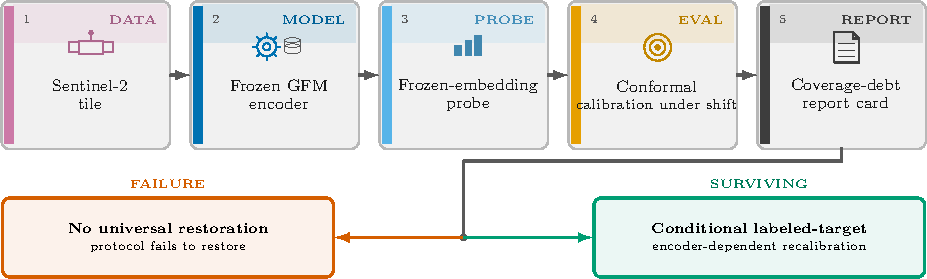
\includegraphics[width=\columnwidth]{fig0_overview.pdf}
\caption{Overview of the pre-deployment reliability report-card protocol.
A Sentinel-2 tile (EuroSAT-MS / GEO-Bench BigEarthNet-S2 / m-so2sat) is
passed through one of the frozen, interchangeable GFM encoders under audit (five illustrated: Prithvi,
Clay, SSL4EO-DINO, SSL4EO-MAE, DOFA) and a frozen-embedding probe (logistic for the single-label tasks,
multi-label otherwise), then conformally calibrated under the real geographic (region-transfer)
shift---source split-conformal vs.\ spatial-Mondrian target-region calibration, source = E/Central Europe,
target = W/Iberian-Atlantic Europe---yielding per-class conformal sets. The protocol reads off four
practitioner-facing numbers for any frozen GFM: the in-distribution FNR guarantee, the geographic debt
under shift, the target-slice repair cost, and the hidden worst-class coverage a marginal guarantee alone
would miss. Vermillion marks the failure path (no universal restoration); bluish green marks the
surviving path (conditional, encoder-dependent labeled-target recalibration).}\label{fig:overview}
\end{figure}
\FloatBarrier

\section{Methods}\label{sec:methods}
The data come from EuroSAT-MS \citep{helber2019eurosat} (Sentinel-2 L2A, 13 bands, 27{,}000 tiles, 10 classes). The shift is a
\emph{real} geographic cross-region holdout using per-tile longitude: source = E/Central Europe
($\mathrm{lon}\ge P_{33}$), target = W/Iberian-Atlantic Europe ($\mathrm{lon}<P_{33}$); no image transform is
applied (Fig.~\ref{fig:geomap}; patch-level examples in Fig.~\ref{fig:geopatches}). The $P_{33}$ cut is a single, fixed longitude-percentile boundary chosen once in advance; a post-hoc
boundary-sensitivity sweep over $P_{25}/P_{40}/P_{50}$ is reported in Results (Table~\ref{tab:boundary};
see Limitations).

\begin{figure}[htbp]
\centering
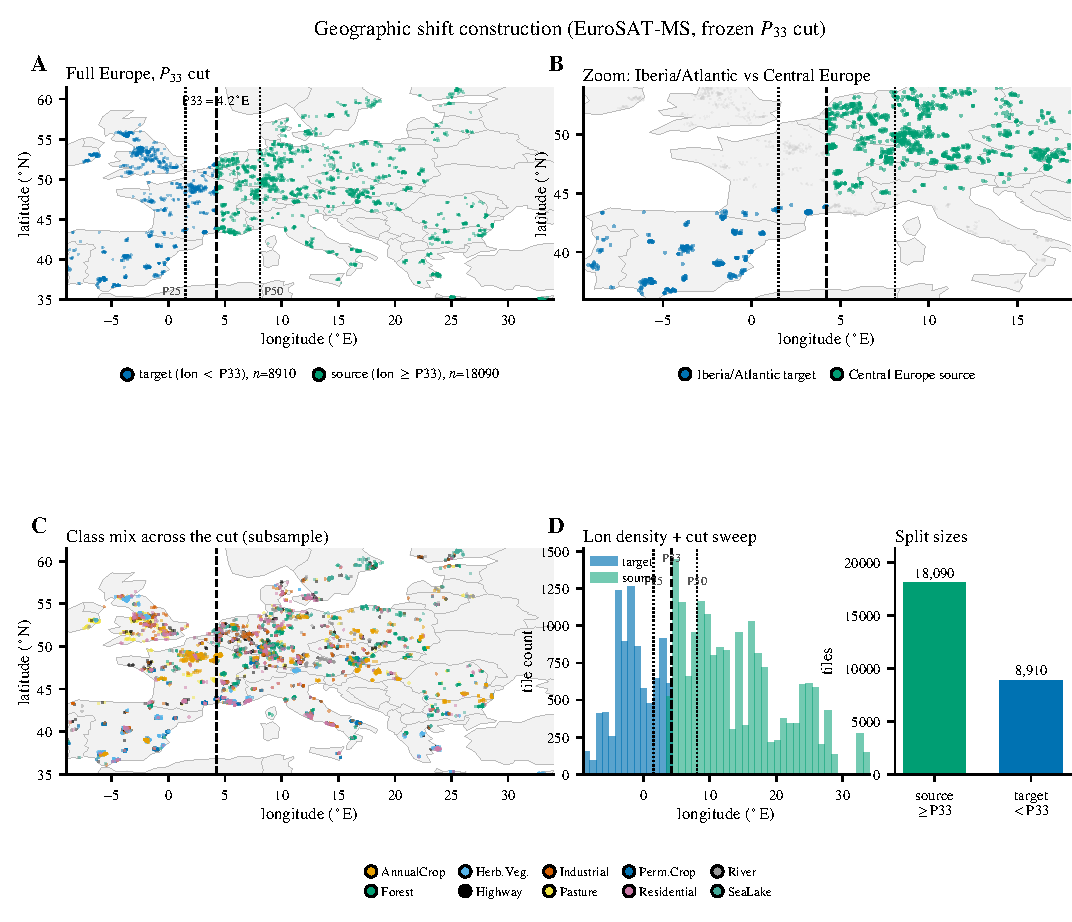
\includegraphics[width=\columnwidth]{F8_geomap.pdf}
\caption{The geographic-shift construction, shown on the map it is defined on: EuroSAT-MS tile
centroids (4{,}000 of 27{,}000, seeded subsample) colored by split side at the $P_{33}$ longitude
cut ($=4.2^\circ$E; $P_{25}$/$P_{50}$ sweep boundaries dotted). Source tiles (E/Central Europe,
$n{=}18{,}090$) calibrate; target tiles (W/Iberian-Atlantic Europe, $n{=}8{,}910$) are the
deployment region. No image transform is applied --- the shift is purely geographic.}
\label{fig:geomap}
\end{figure}

\begin{figure}[htbp]
\centering
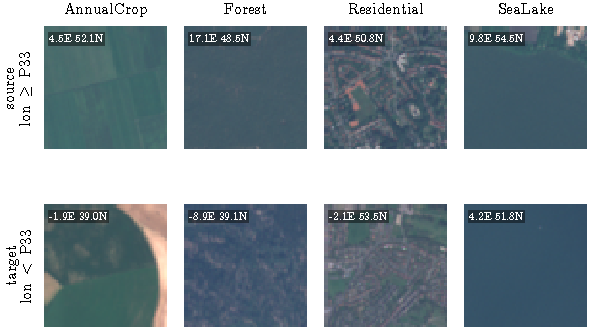
\includegraphics[width=\columnwidth]{F9_geopatches.pdf}
\caption{Geographic shift at patch level: illustrative true-color Sentinel-2 tiles
(seeded selection; tile centroids annotated under each patch) for six land-cover classes
(AnnualCrop, Forest, PermanentCrop, Residential, Highway, SeaLake) under the frozen
$P_{33}$ longitude cut ($=4.2^\circ$E; source $n{=}18{,}090$; target $n{=}8{,}910$).
Rows encode the split sides: source ($\mathrm{lon}\ge P_{33}$), a near-cut boundary band
($|\mathrm{lon}-P_{33}|\le 1.5^\circ$), and target ($\mathrm{lon}<P_{33}$).
Region-specific crop structure, settlement texture, and water color differ systematically across
the cut --- the shift is real but subtle at single-patch level, which is exactly why an
accuracy-only deployment check can miss it.}
\label{fig:geopatches}
\end{figure}
\FloatBarrier

This cut also induces a class-frequency (label-prior) shift
between source and target that we did not adjust for in the headline logistic probe: at $P_{33}$, class~5
% source: experiments/results/eurosat_stage2_multifm_multialpha\slash recompute_class_prior_balanced_control_2026-07-01.json (class_prior_shift_at_P33)
goes from $2.62\%$ of source tiles to $17.13\%$ of target tiles ($6.54\times$ enriched), class~1 from
$15.02\%$ to $3.16\%$ ($\sim\!4.7\times$ depleted), class~8 from $11.60\%$ to $4.51\%$, and class~9 from
$14.10\%$ to $5.04\%$ (remaining classes shift by ${<}2.4\times$; Table~\ref{tab:classprior},
Fig.~\ref{fig:classprior}A--B). We
re-fit the probe with class-balanced sample weighting on the same cached embeddings as a control
(Table~\ref{tab:balanced}, Fig.~\ref{fig:classprior}C--D; see Discussion). The frozen encoders are Prithvi-EO-2.0-300M \citep{szwarcman2024prithvi} (mean-pooled patch tokens, 1024-d); Clay~v1.5 \citep{clay2024model}
(cls token, 1024-d); SSL4EO-S12 \citep{wang2023ssl4eo} ViT-S/16 DINO via torchgeo (cls token, 384-d); SSL4EO-S12 \citep{wang2023ssl4eo} ViT-B/16 MAE
(\texttt{wangyi111/SSL4EO-S12} on HuggingFace, 87.8M params, token-free global pool, 768-d). A fifth
encoder, DOFA (Dynamic One-For-All) \citep{xiong2024dofa}---a ViT-B/16 whose dynamic
wavelength-conditioned patch embedding ingests the Sentinel-2 bands natively (\texttt{dofa\_base\_patch16\_224},
\texttt{DOFA\_MAE} weights via \texttt{torchgeo})---was added on the EuroSAT grid only, frozen and probed
identically. The original four weights loaded strictly (zero missing keys), verified real (in-distribution probe accuracy
% source: experiments/results/eurosat_stage2_multifm_multialpha\slash results.json (accuracy in_dist 0.9524-0.9861; was misstated as 0.95-0.97 in the pre-template draft)
$0.95$--$0.99$ vs.\ chance $0.10$).
% source: GEO-ROSTER-EXPANSION-2026-07-16.md (roster) + roster_analysis_2026-07-16/RESULTS.md (13 scored, 2 dropped)
For the BigEarthNet FNR analysis---the one cross-encoder comparison that turns on statistical power---we
expand this battery to \emph{thirteen} frozen encoders by adding eight more loaded through first-party
trusted paths (\texttt{torchgeo} 0.9.0 built-in weight builders, no third-party repository code
executed), each with normalization read from the weight's own shipped transform: SSL4EO-S12 MoCo
(ViT-S/16, 384-d) and its ResNet50 MoCo/DINO variants (2048-d) \citep{wang2023ssl4eo}; SoftCon
\citep{wang2024softcon} ViT-B/14 (768-d) and ViT-S/14 (384-d); an SSL4EO MAE ViT-L/16 (1024-d); and
CROMA \citep{fuller2023croma} Base (768-d) and Large (1024-d). Two further planned arms
(\texttt{dofa\_large}, \texttt{prithvi\_600m}) were dropped by the pre-specified smoke/mAP gates (missing
or non-finite feature caches at extraction), leaving thirteen scored; the three anchor encoders reused
the frozen caches and reproduce the earlier five-encoder records exactly. The expanded roster is used
only for the BigEarthNet CRC comparison; EuroSAT and m-so2sat retain the five-encoder battery.
A logistic probe is trained on frozen embeddings. We compare source-fit
split-conformal \citep{vovk2005algorithmic,angelopoulos2023conformal} (LAC \citep{sadinle2019lac} nonconformity $1-\hat p_{\text{true}}$) against a \emph{spatial-Mondrian} conformal
predictor \citep{vovk2003mondrian} that draws per-spatial-bin quantiles from a disjoint same-region target-calibration slice. We adopt
the LAC score for its simplicity; adaptive prediction sets \citep{romano2020classification} are a natural
alternative nonconformity score we do not explore. The Mondrian and target-calibration arms rely on
exchangeability within each spatial/target bin, a weaker requirement than global exchangeability; more general
non-exchangeable-shift theory \citep{barber2023conformal} formalizes how conformal coverage can degrade under
shifts broader than the fixed geographic partition studied here, and the conformal-risk-control arm we use
below \citep{angelopoulos2024crc} is itself an instance of the general distribution-free risk-controlling
framework of Bates et al.~\citep{bates2021distributionfree}. We sweep
$\alpha\in\{0.05,0.10,0.20\}$, $5$ seeds, and bootstrap the paired per-seed restoration statistic
$|\text{cov}_{\text{split}}-\text{nom}|-|\text{cov}_{\text{Mondrian}}-\text{nom}|$ (CI${}>0\Rightarrow$ restored).
The set-size cost of that restoration---and the EuroSAT singleton floor it rises above---is reported in
Fig.~\ref{fig:f3}.
A post-hoc boundary-sensitivity sweep repeats the full protocol at $P_{25}/P_{33}/P_{40}/P_{50}$ longitude
cuts on the same cached embeddings, and adds a third, \emph{label-access ablation} arm: non-spatial split
conformal whose single LAC quantile is drawn from the same labeled target-region calibration slice
the Mondrian arm uses (isolating target-label access from spatial conditioning).
All figures (Fig.~\ref{fig:f1}--\ref{fig:f3}, \ref{fig:f5}, \ref{fig:f6},
\ref{fig:geomap}, \ref{fig:geopatches}, \ref{fig:f10}, \ref{fig:condcov},
\ref{fig:singleton}, \ref{fig:crcfnr}, \ref{fig:classprior}) are generated directly from the
frozen result records by the accompanying figure-generation scripts.
As a post-hoc, exploratory extension, after the preregistered gate
(\S\ref{sec:limitations}) we added three decoupling analyses on the same frozen-feature caches, computed
% source: exp0_2026-07-13/RESULTS.md + bigearthnet_crc_2026-07-13/RESULTS.md (reproducer exp0_decoupling.py, lowshot_sweep.py)
from cached embeddings with no GPU re-extraction: (i) on BigEarthNet-S2, a per-encoder comparison
of the CRC arm's shifted FNR against multi-label accuracy (macro mAP) and calibration (mean per-label
ECE) analogs on the same footing (the recomputed shifted FNR reproduces the frozen CRC JSON, e.g.\ Prithvi
$0.129$ vs.\ $0.130$); (ii) on EuroSAT, per-class conditional coverage of the spatial-Mondrian-repaired
target sets at matched marginal coverage ($\approx0.95$--$0.96$), summarized by the worst-class gap
$\big((1{-}\alpha)-\min_k \mathrm{cov}_k\big)$; and (iii) a low-shot sweep that subsamples the
EuroSAT probe-training fraction to $\{0.01,\dots,1.0\}$ and records split set size and the
coverage$-$accuracy gap, mapping the singleton-degeneracy boundary. Correlations across encoders are
Spearman rank statistics ($n{=}13$ FNR on the expanded BigEarthNet roster, $n{=}5$ conditional coverage)
and are reported as directional evidence, not proofs of independence (\S\ref{sec:limitations}).

\section{Results}\label{sec:results}
In plain terms: every frozen encoder loses reliability under a real geographic move, that loss is repaired
only with labeled target-region data, and the sections below map exactly where a conformal audit adds
information beyond accuracy and where it does not.
% ============ RE-CENTERED SPINE (Exp-0 gate, 2026-07-13): the conformal audit is load-bearing through
% (i) multi-label FNR risk control and (ii) per-class conditional coverage -- both dissociate from
% shifted accuracy and shift-ECE -- while the marginal single-label set-size axis is accuracy-restated
% (singleton-degeneracy boundary). The coverage-debt encoder ranking is retained below as secondary.
% source: exp0_2026-07-13/RESULTS.md (gate PASS on Tests B and C; Test A FAIL)
A conformal reliability audit is worth its complexity only if it tells a practitioner
something accuracy and calibration do not, so we lead with the regimes in which it does and with the one
cross-encoder result that is adequately powered. Primary result (next): under a multi-label
false-negative-rate (FNR) risk-control guarantee, all thirteen frozen encoders incur a real geographic FNR
debt that only a labeled target slice repairs, and that debt is bought back with larger prediction sets
(the powered FNR-versus-set-size tradeoff); accuracy itself is only a weak, directional guide to which
encoder is most robust. We then map the audit's validity boundary, a deterministic property: in the
marginal single-label singleton regime the set-size axis is a restatement of accuracy, so EuroSAT at full
data is a mapped negative control, not a decoupling. Next, a remedy-failure result: the textbook unlabeled
covariate-shift fix does not close the debt (its weights' effective sample size collapses), so only a
labeled target-region slice reliably restores the guarantee. As a conditional, single-encoder finding: on
EuroSAT, restoring the \emph{marginal} coverage guarantee hides a per-class conditional-coverage collapse
that neither accuracy nor ECE predicts. Only then do we report the encoder coverage-debt ranking and its
target-side recalibration repair, as a secondary, descriptive diagnostic. Every axis-decoupling analysis
below is post-hoc and exploratory (added after the preregistered gate; \S\ref{sec:limitations}).

\subsection{Primary result: a marginal FNR guarantee incurs a geographic debt no encoder escapes, bought back with larger prediction sets---accuracy is only a weak, directional guide to which encoder is most robust}
% source (n=5, 2026-07-14): box_pulled_2026-07-14/ben_map_n5_2026-07-14.json (per_encoder mAP_in
%   0.4325/0.5021/0.5591/0.5500/0.4585; ece_in 0.0823/0.0783/0.0278/0.0372/0.0571 for
%   prithvi/clay/ssl4eo/ssl4eo_mae/dofa; gate reproduces frozen 0.4325/0.5023/0.5589 to <=2.4e-4)
%   + experiments/results/bigearthnet_crc_arm-exec-2026-06-29.json (n=5 box run; per_alpha 0.05
%   fnr_sh_crc 0.1300/0.1762/0.1905/0.1695/0.1692; fnr_sh_mond 0.031/0.022/0.032/0.030/0.021;
%   ss_sh_crc 15.5/13.3/10.6/11.8/13.0). Decoupling 0.05 (n=5): spearman fnr_vs_mAP +0.90 (p=0.037,
%   9/10 inversions), fnr_vs_ece -0.70, fnr_vs_ss -0.70. See box_pulled_2026-07-14/GEO-N5-DIGEST.md.
% ECE per-seed spread: exp0_2026-07-13/worstclass_uncertainty_2026-07-14.json item3 (prithvi ece 0.0823 std 0.0019, clay 0.0783 std 0.0032; paired delta 0.004, per-seed std 0.0019, delta>seed-noise TRUE, prithvi worse-calibrated in every seed; FNR gap 0.046)
On GEO-Bench \texttt{m-bigearthnet} (BigEarthNet-S2; $7{,}669$ tiles, $39$ active labels; real E$\to$W
geographic shift), a conformal-risk-control (CRC) predictor \citep{angelopoulos2024crc} bounds the
example-averaged FNR---a set-valued guarantee with \emph{no top-1-accuracy analog by construction}.
We audit \emph{thirteen} frozen encoders here (the five-encoder battery plus eight added at pull
expressly to power the cross-encoder comparison; roster in \S\ref{sec:methods}).
The within-encoder finding is unambiguous and requires no cross-encoder statistics: for \emph{every one}
of the thirteen encoders, source-calibrated CRC meets the target FNR in-distribution ($0.051$--$0.056$ at
$\alpha{=}0.05$) yet incurs a real FNR debt under shift ($0.130$ Prithvi to $0.234$ ResNet50-MoCo, i.e.\
$2.6$--$4.7\times$ nominal across the whole roster), which a target-side Mondrian-CRC arm repays
($0.002$--$0.036$; Table~\ref{tab:fnrdecouple}, full per-$\alpha$ CRC/repair numbers in
Table~\ref{tab:crc}). Unlike the inert EuroSAT-singleton regime (validity-boundary result below), the
repair is active here. This debt-and-repair is the reliability-relevant result: the marginal guarantee a
practitioner would trust degrades under a regional move---uniformly, across every backbone we tested---and
is restored only with a labeled target-region slice.
% source: roster_analysis_2026-07-16/population_test.py -> population_test.json (n=13, nominal=0.05,
%   alpha arm 0.05; debt_direction/repair_direction n_successes=13/13; sign_test_two_sided_p=2.44e-4,
%   one_sided_p=1.22e-4; wilcoxon one-sided p=1.22e-4 for both directions; bootstrap-CI exclusion 13/13
%   both directions). Computed over roster_pulled_2026-07-16/bigearthnet_crc_arm_roster_2026-07-16.json.
This pattern is not merely descriptive: treating the thirteen preregistered per-encoder point estimates
as a population, a distribution-free sign test confirms that shifted CRC FNR exceeds the nominal target
in all thirteen encoders (two-sided $p\approx2.4\times10^{-4}$) and that target-side Mondrian-CRC returns
FNR to at or below nominal in all thirteen (same test, same $p$); a Wilcoxon signed-rank sensitivity
check agrees exactly (one-sided $p\approx1.2\times10^{-4}$ for both directions, the smallest value
attainable at $n{=}13$), and every one of the thirteen per-encoder bootstrap confidence intervals
excludes nominal in the claimed direction, for both the debt and the repair arm. We report the
one-sided figure only as a sensitivity check: the debt-and-repair direction was not discovered in this
roster run but inherited from the original five-encoder confirmatory arm, so it is defensible, but the
two-sided value is what we use as the headline since it needs no such defense and is already decisive.
This is a population-level summary computed post-hoc over the frozen, preregistered per-encoder
estimates---the per-encoder numbers are prereg and frozen, but the population test itself is not---and
it supplies a second firm, statistically-tested positive result alongside the preregistered
falsification of universal restoration (\S\ref{sec:limitations}). Two further qualifications
bound what the test shows. First, the thirteen encoders share the same target-shift
BigEarthNet split and labels, so this is a distribution-free summary over thirteen
preregistered per-encoder point estimates, not an i.i.d.-sample hypothesis test: the nominal
$p$ treats the sign pattern combinatorially, and shared-target dependence means the effective
number of independent draws is smaller than thirteen. Second, the repair-arm direction is what
the target-calibrated Mondrian-CRC guarantee is constructed to deliver, so its $13/13$ reads
as a verification that the guarantee holds in practice rather than as an independent discovery.
% source: roster_analysis_2026-07-16/population_test_family.py -> population_test_family.json
%   (n_families=6, grouping: ssl4eo_s12-pretrained ViT/ResNet variants as one family, SoftCon and
%   CROMA each one family across their B/L or B/S variants, Prithvi/Clay/DOFA singleton families;
%   family vote = unanimous within-family agreement; debt/repair n_family_successes=6/6,
%   sign_test_two_sided_p=0.03125, one_sided_p=0.015625)
Re-aggregating to the level of independent encoder families---encoders sharing a pretraining
corpus and method lineage (all six SSL4EO-S12-pretrained ViT/ResNet variants as one family; SoftCon
and CROMA each one family across their two size variants; Prithvi, Clay, and DOFA as singleton
families, six families in total) and requiring unanimous within-family agreement, the most
conservative vote rule available---still gives a unanimous $6/6$ sign test in both directions, but
at a far weaker two-sided $p\approx0.031$ (one-sided $p\approx0.016$): the family-clustered
correction survives at $\alpha{=}0.05$, but only barely, so the thirteen per-encoder bootstrap
confidence intervals (all excluding nominal in the claimed direction) remain the primary evidence,
not the population $p$-value at either $n$.

The one adequately powered cross-encoder result is a risk-versus-efficiency tradeoff: FNR robustness is
bought with larger prediction sets
($\mathrm{Spearman}(\mathrm{FNR}_{\mathrm{sh}},\text{set size})=-0.33$ at $\alpha{=}0.05$, $-0.66$
($p{=}0.017$) at $\alpha{=}0.10$; Prithvi buys the best FNR with the largest sets, $15.5$ labels/tile)---an
operating-point choice a practitioner can act on directly, independent of which encoder they picked.

Does accuracy also tell a practitioner \emph{which} encoder to trust? Here the evidence is weaker, and we
report it as directional context rather than a claim. The FNR under shift is only weakly rank-correlated
with in-distribution mAP
($\mathrm{Spearman}(\mathrm{FNR}_{\mathrm{sh}},\mathrm{mAP})=+0.32$, permutation $p{=}0.28$, $n{=}13$,
$\alpha{=}0.05$; Fig.~\ref{fig:inv13}) and not at all with calibration
($\mathrm{Spearman}(\mathrm{FNR}_{\mathrm{sh}},\mathrm{ECE}_{\mathrm{in}})=-0.16$, $p{=}0.60$). The
correlation is \emph{positive}---higher accuracy never buys better FNR robustness, and the ordering never
reverses to ``better encoder $\to$ better reliability''---but it does not reach significance and $48$ of
$78$ encoder pairs ($62\%$) invert, so we do \emph{not} claim a strong accuracy-to-reliability inversion;
at $n{=}13$ this is a weak, directional statement, not proof that accuracy is uninformative. One extreme
survives the expansion and carries the practical point: Prithvi, the least accurate encoder (mAP
$0.432$), is the \emph{most} FNR-robust ($0.130$), while the two most FNR-fragile encoders---the ResNet50
CNNs (MoCo/DINO, $0.234$/$0.232$)---sit mid-pack on accuracy; and Prithvi vs.\ Clay is a
near-calibration-matched dissociation (ECE $0.082$ vs.\ $0.078$, differing by $0.004$, yet FNR $0.130$
vs.\ $0.176$, the worse-calibrated encoder holding the better FNR). In those first five encoders the same
mAP-correlation statistic read $+0.90$ (asymptotic $p{=}0.037$; its \emph{exact} permutation $p$ was
already $0.083$); the roster expansion regresses it toward zero, precisely the power test the expansion
was run to perform, and we report the weakened result rather than the headline it displaced
(\S\ref{sec:limitations}).

\begin{table*}[!t]\centering\small
\caption{Primary decoupling on GEO-Bench \texttt{m-bigearthnet} ($\alpha{=}0.05$; $13$ frozen encoders,
sorted by mAP): every encoder meets the target FNR in-distribution and incurs a $2.6$--$4.7\times$ FNR
debt under shift that the target-side Mondrian-CRC arm repairs. ``FNR shift'' is the source-calibrated
CRC arm's shifted FNR; ``repaired'' is the target-side Mondrian-CRC arm; set size is CRC labels/tile under
shift. Accuracy is a weak, non-significant guide to FNR robustness:
$\mathrm{Spearman}(\mathrm{FNR}_{\mathrm{sh}},\mathrm{mAP})=+0.32$ ($p{=}0.28$; $48/78$ inversions),
$(\mathrm{FNR}_{\mathrm{sh}},\mathrm{ECE})=-0.16$ ($p{=}0.60$),
$(\mathrm{FNR}_{\mathrm{sh}},\text{set size})=-0.33$ ($n{=}13$; $-0.66$, $p{=}0.017$ at
$\alpha{=}0.10$).}\label{tab:fnrdecouple}
\begin{tabular}{lccccc}
\toprule
Encoder & mAP (in) & ECE (in) & FNR shift & FNR repaired & Set size \\
\midrule
% source: roster_analysis_2026-07-16/results.json (per_alpha 0.05 rows) = ben_map_roster_2026-07-16.json
%   (mAP_in, ece_in) + bigearthnet_crc_arm_roster_2026-07-16.json (fnr_sh_crc / fnr_sh_mond / ss_sh_crc
%   bootstrap means). Anchor rows (Prithvi/Clay/SSL4EO-DINO) reproduce the frozen n=5 records exactly.
Prithvi              & 0.432 & 0.082 & 0.130 & 0.031 & 15.5 \\
DOFA                 & 0.459 & 0.057 & 0.169 & 0.021 & 13.0 \\
Clay                 & 0.502 & 0.078 & 0.176 & 0.022 & 13.3 \\
SoftCon-ViT-B        & 0.525 & 0.033 & 0.174 & 0.031 & 11.9 \\
SoftCon-ViT-S        & 0.525 & 0.020 & 0.213 & 0.036 & 10.7 \\
CROMA-L              & 0.541 & 0.037 & 0.169 & 0.024 & 11.6 \\
CROMA-B              & 0.544 & 0.046 & 0.182 & 0.030 & 12.1 \\
ResNet50-MoCo        & 0.548 & 0.073 & 0.234 & 0.002 & 12.5 \\
SSL4EO-MAE           & 0.550 & 0.037 & 0.170 & 0.030 & 11.8 \\
SSL4EO-MAE (ViT-L)   & 0.550 & 0.038 & 0.155 & 0.029 & 11.9 \\
ResNet50-DINO        & 0.551 & 0.055 & 0.232 & 0.014 & 10.8 \\
SSL4EO-DINO          & 0.559 & 0.028 & 0.191 & 0.032 & 10.6 \\
SSL4EO-MoCo          & 0.582 & 0.032 & 0.171 & 0.028 & 10.7 \\
\bottomrule
\end{tabular}
\end{table*}

\begin{figure}[htbp]\centering
\includegraphics[width=\columnwidth]{F7_ben_inversion_n13.pdf}
\caption{The five-encoder inversion does not survive expansion to thirteen. FNR under shift vs.\
in-distribution mAP on \texttt{m-bigearthnet} ($\alpha{=}0.05$, CRC arm); circles are the original five
encoders, triangles the eight added at pull. The rank correlation is a weak, non-significant positive
($\mathrm{Spearman}=+0.32$, permutation $p{=}0.28$, $n{=}13$; no trend line is drawn, since the
correlation does not reach significance): accuracy
never buys better FNR robustness, but the strong $+0.90$ inversion of the five-encoder slice regresses
toward zero. Prithvi (least accurate) remains the most FNR-robust; the two ResNet50 CNNs are the most
fragile at mid accuracy.}\label{fig:inv13}\end{figure}
\FloatBarrier

\subsection{Secondary (conditional) result: marginal coverage repair hides a per-class conditional collapse}
% source: exp0_2026-07-13/results.json test_B_eurosat_conditional_coverage per_alpha 0.05
%   (worst_class_gap prithvi 0.0455/clay 0.0481/ssl4eo 0.0999/ssl4eo_mae 0.0378/dofa 0.0305;
%    worst_class_cov ssl4eo 0.8501 under marg_cov 0.9558; spearman worstgap_vs_acc +0.30 p=0.62,
%    vs_ece -0.30 p=0.62, partial acc|ece -0.034; 6/10 inversions; alpha 0.10 ssl4eo worst 0.7762 under 0.9255)
% per-seed spread: exp0_2026-07-13/worstclass_uncertainty_2026-07-14.json item2 ssl4eo (worst class id=3 in all 5 seeds; per-seed worst-class cov [0.839,0.826,0.858,0.856,0.871], min 0.826 max 0.871 std 0.016, seed-avg 0.850)
After the target-side spatial-Mondrian arm restores the \emph{marginal} EuroSAT guarantee to
$\approx0.95$--$0.96$ for every encoder (secondary results below), we ask what that marginal scalar hides:
how badly does the worst individual land-cover class still under-cover? At matched marginal coverage
($\alpha{=}0.05$, 5 seeds; Table~\ref{tab:condcov}; Fig.~\ref{fig:condcov}) the worst-class gap is scrambled relative to
accuracy and ECE---$\mathrm{Spearman}(\text{worst gap},\text{acc})=+0.30$ ($p{=}0.62$),
$\mathrm{Spearman}(\text{worst gap},\text{ECE})=-0.30$ ($p{=}0.62$), $6$ of $10$ pairwise inversions
against each, partial correlation $\approx0$ ($-0.03$ for acc$\mid$ece). The smoking gun: SSL4EO-DINO is
mid-pack on accuracy ($0.880$, 3rd of 5) and ECE ($0.076$, 3rd) yet silently abandons a class---one
EuroSAT class is covered at only $0.850$ under a $0.956$ marginal (a $0.106$ within-encoder conditional
shortfall, $2\times$ the next-worst encoder's gap), and it is the same class that under-covers in all
five seeds (per-seed coverage $0.826$--$0.871$, std $0.016$; the datum is seed-stable, not a single-seed
artifact). Nothing in its accuracy or calibration predicts this:
DOFA, the second-least accurate encoder ($0.851$), has the best conditional coverage (gap
$0.031$), while Clay---the most accurate ($0.918$) and best-calibrated (ECE $0.057$)---has the
second-worst (gap $0.048$). The effect sharpens at $\alpha{=}0.10$, where SSL4EO-DINO's worst class
sits at $0.776$ under a $0.926$ marginal. Which frozen encoder quietly drops a class under geographic shift
is invisible to accuracy and to ECE and is surfaced only by the conditional conformal audit. Honest
caveat: $n{=}5$ gives low power---all $p>0.28$ and the weak rank correlation even flips sign across
$\alpha$---so the claim is ``no detectable/stable dependence plus large concrete inversions,'' not proven
independence; the SSL4EO-DINO case is the load-bearing single datum and is reported as such
(\S\ref{sec:limitations}).

\begin{table*}[!t]\centering\small
\caption{Per-class conditional coverage of the marginally repaired EuroSAT predictor
(spatial-Mondrian, $\alpha{=}0.05$; marginal coverage matched to $\approx0.95$--$0.96$; 5 seeds). The
worst-class gap does not track accuracy or ECE ($\mathrm{Spearman}=+0.30/-0.30$, $p{=}0.62$; $6/10$
inversions). SSL4EO-DINO, mid-pack on both scalars, abandons a class at $0.850$ (seed-stable; range $0.826$--$0.871$); the most accurate and
best-calibrated encoder (Clay) has the second-worst gap. Accuracy/ECE columns are the canonical shift
values; the conditional columns are the exp0 recompute.}\label{tab:condcov}
\begin{tabular}{lccccc}
\toprule
Encoder & Acc.\ shift & ECE shift & Marg.\ cov & Worst-class cov & Worst gap (vs.\ nominal) \\
\midrule
% source: exp0_2026-07-13/results.json test_B per_alpha 0.05 (marg_cov/worst_class_cov/worst_class_gap);
%   acc/ECE = canonical experiments/results/eurosat_stage2_multifm_multialpha/results.json real_shift
DOFA        & 0.851 & 0.093 & 0.951 & 0.919 & 0.031 \\
SSL4EO-MAE  & 0.898 & 0.065 & 0.962 & 0.912 & 0.038 \\
Prithvi     & 0.833 & 0.109 & 0.955 & 0.905 & 0.045 \\
Clay        & 0.918 & 0.057 & 0.960 & 0.902 & 0.048 \\
SSL4EO-DINO & 0.880 & 0.076 & 0.956 & 0.850 & 0.100 \\
\bottomrule
\end{tabular}
\end{table*}

\begin{figure*}[htbp]\centering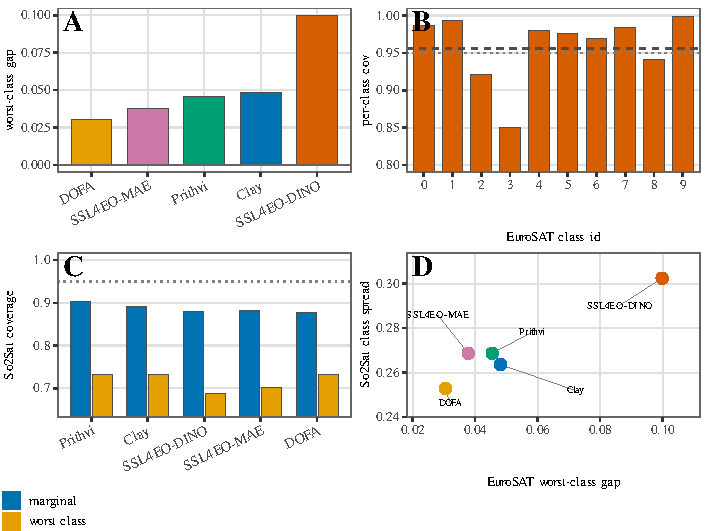
\includegraphics[width=0.95\textwidth]{F11_conditional_coverage.pdf}
\caption{Conditional-coverage panels from the frozen EuroSAT and So2Sat roster summaries
(no new runs; $\alpha{=}0.05$).
(A)~EuroSAT worst-class coverage gap $G_{\mathrm{worst}}$ by encoder (Okabe--Ito colours).
(B)~SSL4EO-DINO per-class conditional coverage on EuroSAT (dashed $=$ encoder marginal;
dotted $=$ nominal $0.95$).
(C)~So2Sat source-only split coverage by encoder: marginal (blue) vs.\ worst class (gold);
dotted $=$ nominal $0.95$.
(D)~Encoder scatter of EuroSAT worst-class gap vs.\ So2Sat class-coverage spread
(same encoder colours as~(A)).
}\label{fig:condcov}\end{figure*}
\FloatBarrier

\subsection{The audit's validity boundary: singleton degeneracy of the marginal single-label set}
% source: exp0_2026-07-13/results.json test_A (eurosat_mondrian_n5 0.05: spearman ss_vs_acc -1.0,
%   ss_vs_ece +1.0, zero inversions) + lowshot_results.json (prithvi 0.05 singleton transition)
A conformal set-size axis can decouple from accuracy only where the sets are non-trivial. On EuroSAT at
full data the source-calibrated split predictor emits \emph{singletons} on the shifted target (mean set
size $1.00$ for every encoder and $\alpha$; per-seed $\le1.001$; Fig.~\ref{fig:f3}b), so its coverage coincides with shifted
top-1 accuracy (5-seed-mean $|\Delta|\le2\times10^{-4}$) and the marginal set-size/efficiency axis carries
no information beyond accuracy. Even after target-side repair the restored Mondrian set size is a
deterministic image of accuracy loss (Fig.~\ref{fig:f3}a): across the five encoders $\mathrm{Spearman}(\text{set size},\text{acc})=-1.0$
and $\mathrm{Spearman}(\text{set size},\text{ECE})=+1.0$ ($\alpha{=}0.05$, zero pairwise inversions). We
therefore report set size only as a companion to a held guarantee, never as evidence that the conformal
layer beats accuracy---the preregistered ``efficiency-decoupling'' route is empirically falsified on this
benchmark and we say so.
% source: exp0_2026-07-13/lowshot_results.json (prithvi 0.05: frac 1.0 acc0.832 ss1.000 gap0.000 ... frac0.01 acc0.650 ss2.294 gap0.221; clay singleton by acc~0.87, ssl4eo by acc~0.82)
Mapping the boundary. Subsampling the probe-training fraction drives shifted accuracy down and
locates where the audit switches from degenerate to informative (Table~\ref{tab:singleton},
Fig.~\ref{fig:singleton}). In the
high-accuracy regime (acc $\gtrsim0.80$ at $\alpha{=}0.05$) sets are exact singletons (size $\equiv1.000$)
and coverage $\equiv$ accuracy; as the task hardens below acc $\approx0.78$ the sets go non-singleton
(size $>1.05$) and the coverage$-$accuracy gap opens from $0$ to $+0.22$. The more accurate the encoder,
the higher the accuracy at which it degenerates (Clay singleton by acc $\approx0.87$, SSL4EO-DINO by
$\approx0.82$). This makes EuroSAT at full data an explicit negative control: it sits above
the boundary, so its \emph{marginal} single-label audit is accuracy-restated---which is precisely why the
per-class conditional audit above (on the non-singleton repaired sets) and the multi-label FNR audit
on BigEarthNet are where the conformal layer earns its keep, and why So2Sat (17-class LCZ, shifted accuracy
$0.52$--$0.60$), which sits below the boundary, carries informative non-singleton sets even
marginally (Table~\ref{tab:so2sat}). The boundary is itself a contribution: it tells a practitioner when a
marginal conformal audit of a frozen GFM is worth running.

\begin{table*}[!t]\centering\small
\caption{Singleton-degeneracy boundary (EuroSAT, Prithvi, $\alpha{=}0.05$, 3 seeds): subsampling the
probe-training fraction lowers shifted accuracy and moves the split predictor from degenerate (singletons,
coverage $\equiv$ accuracy) to informative (non-singleton sets, coverage decoupled from accuracy). The
transition sits near accuracy $\approx0.78$--$0.80$.}\label{tab:singleton}
\begin{tabular}{lcccc}
\toprule
Train frac & Train $n$ & Shifted acc & Split set size & Coverage $-$ accuracy \\
\midrule
% source: exp0_2026-07-13/lowshot_results.json (encoders.prithvi."0.05")
1.00 & 10854 & 0.832 & 1.000 & $+0.000$ \\
0.50 & 5427  & 0.805 & 1.026 & $+0.011$ \\
0.25 & 2713  & 0.783 & 1.072 & $+0.026$ \\
0.10 & 1085  & 0.765 & 1.202 & $+0.066$ \\
0.05 & 542   & 0.721 & 1.383 & $+0.107$ \\
0.02 & 217   & 0.645 & 1.866 & $+0.196$ \\
0.01 & 108   & 0.650 & 2.294 & $+0.221$ \\
\bottomrule
\end{tabular}
\end{table*}

\begin{figure*}[!htbp]\centering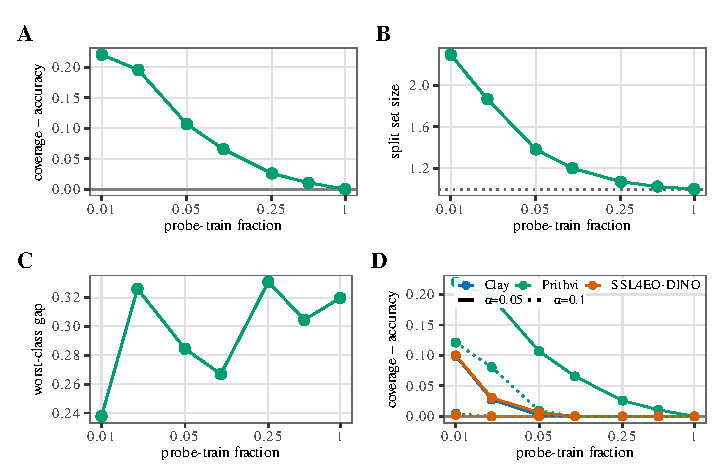
\includegraphics[width=0.95\textwidth]{F12_singleton_lowshot.pdf}
\caption{Singleton / low-shot validity boundary from the frozen EuroSAT
low-shot sweep (no new runs).
Panels~(A)--(C) show the Prithvi series at $\alpha{=}0.05$ vs.\ probe-train fraction
(log-$x$).
(A)~Coverage$-$accuracy gap: as the budget rises, gap$\to0$ and coverage collapses onto
accuracy (degenerate regime).
(B)~Mean split set size on the same $x$-axis---a \emph{different} quantity from~(A), not a
restatement of the gap; the dotted line at size~$=1$ is the singleton floor.
(C)~Worst-class coverage gap vs.\ fraction (conditional residual under the same sweep).
(D)~Multi-encoder comparison (Clay, Prithvi, SSL4EO-DINO): coverage$-$accuracy vs.\ fraction
with colour $=$ encoder and linestyle solid~$\alpha{=}0.05$ / dotted~$\alpha{=}0.10$.
Panels~(A) and~(B) are related through the singleton transition but are not redundant:
gap measures coverage--accuracy decoupling, while set size measures how large the prediction
sets become once that decoupling appears.
}\label{fig:singleton}\end{figure*}
\FloatBarrier

\subsection{Secondary descriptive: the coverage-debt encoder ranking and its target-side repair}
The remaining EuroSAT results are the coverage-debt ranking and target-recalibration repair. They are a
useful descriptive diagnostic but, per the validity-boundary result above, the marginal ranking coincides
with the shifted-accuracy ranking; we report them as such, not as an independent conformal signal.
% source: experiments/results/eurosat_stage2_multifm_multialpha\slash results.json (accuracy: 0.9524->0.8328 prithvi, 0.9724->0.8799 ssl4eo, 0.9777->0.9182 clay; ece real_shift 0.1087/0.0757/0.0650/0.0566)
Coverage debt is real and encoder-dependent: under shift, accuracy drops $0.95\to0.83$ (Prithvi),
$0.97\to0.88$ (SSL4EO-DINO), $0.98\to0.92$ (Clay), and ECE rises to $0.109$ (Prithvi),
$0.076$ (SSL4EO-DINO), $0.065$ (SSL4EO-MAE), $0.057$ (Clay)---an ordering of calibration degradation across
the four encoders that is preserved under the boundary sweep (Table~\ref{tab:boundary};
Fig.~\ref{fig:f1}C) and the
class-prior-balanced probe control (Discussion), so it does not rest on a bare four-point monotonicity
(Fig.~\ref{fig:f1}A--B). As a continuous, bucket-free debt measure we integrate the target coverage gap
$\max(0,(1-\alpha)-\mathrm{cov}_{\mathrm{split}})$ over the $\alpha$ sweep:
% source: experiments/results/eurosat_stage2_multifm_multialpha\slash results.json (integrated coverage-gap debt, trapezoid over alpha in {0.05,0.10,0.20}: prithvi 8.0e-3, ssl4eo 3.3e-3, ssl4eo_mae 1.4e-3, clay 0.8e-3)
% source: experiments/results/eurosat_stage2_multifm_multialpha\slash DOFA-SUMMARY-corrected-2026-07-13.json (CORRECTED 768-d embedding; shift_split_cov 0.8507 at alpha 0.05/0.10/0.20; trapezoid gap-integral D approx 6.2e-3, second-heaviest: Prithvi 8.0 > DOFA 6.2 > SSL4EO-DINO 3.3; supersedes buggy 45-d-head-logit DOFA-SUMMARY-2026-07-12.json)
$D = 8.0 / 3.3 / 1.4 / 0.8 \times 10^{-3}$ for Prithvi\,/\,SSL4EO-DINO\,/\,SSL4EO-MAE\,/\,Clay---and $D\approx6.2\times10^{-3}$ for DOFA, added on the same grid as a fifth encoder and the second-heaviest debt, between Prithvi and SSL4EO-DINO---recovering the
same ordering without the coarse $k/3$ repaired-levels bucketing. The gap closes at $\alpha=0.20$ for all
five encoders because shifted accuracy already meets the $0.80$ nominal---a no-debt artifact of the
easy risk level, not evidence of a repair. DOFA's shifted split coverage is $0.851$ at every risk level, so
like the four battery encoders it carries under-coverage debt only at $\alpha=0.05$ and $0.10$.

% source: experiments/results/eurosat_stage2_multifm_multialpha\slash results.json (alpha 0.05: split 0.8330/0.8799/0.8984/0.9182; mondrian 0.9547/0.9560/0.9621/0.9602; set size 1.619/1.434/1.393/1.223)
% source: experiments/results/eurosat_stage2_multifm_multialpha\slash DOFA-SUMMARY-corrected-2026-07-13.json (CORRECTED 768-d embedding; dofa 5th encoder, alpha 0.05/0.10/0.20: indist split 0.9655; shift split 0.8507; shift+mondrian 0.9506/0.9135/0.8730 at set size 1.5839/1.2875/1.0807; restored 2/3 (alpha 0.05,0.10) by paired-seed CI-excludes-0; overall_verdict KILL = multi-FM gate artifact, clay/prithvi absent from single-FM call; supersedes buggy 45-d-head-logit DOFA-SUMMARY-2026-07-12.json)
Spatial-Mondrian repays the debt where it exists: at $\alpha=0.05$ (nominal $0.95$), source
split-conformal under-covers ($0.833$ Prithvi, $0.851$ DOFA, $0.880$ SSL4EO-DINO, $0.898$ SSL4EO-MAE,\footnote{%
SSL4EO-MAE's shifted split coverage is $0.8984$ in this five-encoder run (shown as $0.898$) and $0.8985$ in the
covariate- and label-shift baseline runs (Tables~\ref{tab:weighted}--\ref{tab:labelshift}, shown as $0.899$);
the ${<}10^{-4}$ difference is independent calibration-split RNG on the same cached features, and split coverage
equals shifted top-1 accuracy in every case (singleton sets).} $0.918$ Clay)
while spatial-Mondrian restores coverage to $0.955$, $0.951$, $0.956$, $0.962$, and $0.960$ respectively,
with paired-bootstrap CI excluding $0$ for all five encoders (Fig.~\ref{fig:f2}). The magnitude of repair tracks the debt:
at this shared risk level the restoration set size is monotone in debt---$1.62$ (Prithvi) $>$ $1.58$ (DOFA) $>$ $1.43$
(SSL4EO-DINO) $>$ $1.39$ (SSL4EO-MAE) $>$ $1.22$ (Clay) (Fig.~\ref{fig:f3}).
The number of risk levels repaired is weakly monotone: Prithvi (heaviest debt) and DOFA (second-heaviest) are each repaired at $2/3$
levels ($\alpha=0.05,0.10$), while SSL4EO-DINO, SSL4EO-MAE, and Clay are each repaired at $1/3$ ($\alpha=0.05$). At
$\alpha=0.20$ (nominal $0.80$) none of the five is repaired because shifted accuracy ($0.83$--$0.92$, DOFA $0.85$) already meets
nominal---there is no under-coverage debt to repay, and the correction correctly does nothing
(Fig.~\ref{fig:f2}). DOFA was added to the same EuroSAT grid as a fifth encoder in a single-FM run whose
spatial-Mondrian set sizes are $1.58/1.29/1.08$ at $\alpha=0.05/0.10/0.20$; an aggregate fail under the
multi-encoder universal-restoration rule is expected here (Clay and Prithvi were absent from that single-encoder call), while the per-encoder
outcome is restoration at $\alpha=0.05$ and $0.10$ by the same paired-bootstrap CI-excludes-$0$ test applied to
the four battery encoders (paired gap-difference CI low $>0$), and no repair at $\alpha=0.20$, where DOFA already
over-covers ($0.851$). Correction note: this DOFA arm was re-run after an initial run
inadvertently probed DOFA's $45$-way classification-head output instead of
its $768$-d pooled feature embedding; all DOFA numbers reported here are from the corrected
embedding run, with the incorrect probe outputs archived for provenance. The four battery encoders are
% source: experiments/results/labelshift_adjusted_baseline/results.json feature_dim (prithvi 1024, clay 1024, ssl4eo/DINO 384, ssl4eo_mae 768); the 45-d head-logit signature appears in no other feature cache
unaffected: their cached features were verified at their documented embedding widths (Prithvi and Clay
$1024$-d, SSL4EO-DINO $384$-d, SSL4EO-MAE $768$-d), and the bug's $45$-dimensional signature appears in no
other feature cache.

% source: experiments/results/eurosat_stage2_multifm_multialpha\slash results.json (real_shift ece raw 0.109/0.076/0.065/0.057 -> ece_tempscaled_srcT 0.058/0.041/0.054/0.032; in_dist ece 0.026/0.014/0.005/0.013, 5-seed means)
Temperature scaling \citep{guo2017calibration} proves insufficient: applying the source-fit temperature to the shifted logits
lowers ECE to $0.058/0.041/0.054/0.032$ (Prithvi/SSL4EO-DINO/SSL4EO-MAE/Clay) from the raw
$0.109/0.076/0.065/0.057$, but the residual still sits $2$--$11\times$ above the in-distribution level
($0.026/0.014/0.005/0.013$), motivating the distribution-free conformal route; a focal-loss-based
calibration alternative \citep{mukhoti2020calibrating} is likewise post-hoc-parametric and is not explored here.

% source: experiments/results/eurosat_boundary_sweep/results.json (ece_real_shift prithvi 0.144/0.108/0.103/0.093, clay 0.074/0.057/0.051/0.041; split coverage prithvi 0.792->0.859; 15/16 restoration cells, exception clay P50 split 0.936)
The headline is not a single-cut artifact: sweeping the source/target
longitude cut over $P_{25}/P_{33}/P_{40}/P_{50}$ on the same cached embeddings (5 seeds each;
Table~\ref{tab:boundary}) preserves the shift-ECE encoder ordering Prithvi $>$ SSL4EO-DINO $>$ SSL4EO-MAE
$>$ Clay at every boundary (Prithvi $0.144/0.108/0.103/0.093$ vs.\ Clay $0.074/0.057/0.051/0.041$ at
$P_{25}/P_{33}/P_{40}/P_{50}$), and the debt shrinks monotonically as the cut moves east and the target
becomes less extreme (Prithvi split coverage $0.792\to0.859$). The ordering is over a small roster (five
% source: experiments/results/eurosat_boundary_sweep/results.json (P25 shift-ECE a=0.05: ssl4eo/DINO 0.0950 vs ssl4eo_mae/MAE 0.0936, gap 0.0014)
encoders at $P_{33}$, four across the sweep) and some adjacent gaps sit within seed noise---e.g.\ SSL4EO-DINO
and SSL4EO-MAE differ by only ${\approx}0.001$ shift-ECE at $P_{25}$---so the extremes (Prithvi heaviest, Clay
lightest) are robust while adjacent mid-rank ties should not be over-interpreted. At $\alpha=0.05$, Mondrian restoration
(paired-seed CI excluding $0$) holds in $15$ of $16$ encoder$\times$boundary cells; the sole exception is
Clay at $P_{50}$, where split coverage is already $0.936$ (debt ${\approx}0.014$)---exactly the
debt-targeted behaviour the conditional framing predicts. At $\alpha=0.10$, Prithvi (heaviest debt) is
restored at all four boundaries while the lighter-debt encoders mostly are not.

% source: experiments/results/eurosat_boundary_sweep/results.json (conformal_target_global coverage 0.946-0.952 at alpha=0.05; target_global_minus_mondrian ci_excludes_0_positive in 0/48 cells; split_minus_target_global in 22/48; set sizes at P33 alpha=0.05: mond 1.621/1.436/1.394/1.224 vs tg 1.563/1.297/1.202/1.116)
A label-access ablation shows that target calibration, not spatial binning, is the active ingredient: the
non-spatial target-calibrated arm restores coverage to $0.946$--$0.952$ at $\alpha=0.05$ in every debt
cell---statistically indistinguishable from spatial-Mondrian: the paired-seed ``Mondrian minus
target-global'' gap-reduction CI excludes $0$ in zero of $48$ (FM$\times$boundary$\times\alpha$)
cells, while target-global itself beats source-only split-conformal in the $22$ cells where debt exists.
Mondrian's set sizes are consistently larger ($P_{33}$, $\alpha=0.05$: $1.62$ vs.\ $1.56$ Prithvi;
$1.44$ vs.\ $1.30$ SSL4EO-DINO; $1.39$ vs.\ $1.20$ SSL4EO-MAE; $1.22$ vs.\ $1.12$ Clay). On this benchmark
and $4\times4$ grid, then, the repair is bought by access to labeled target-region calibration data;
per-spatial-bin conditioning adds no measurable marginal coverage benefit. We report this honestly and
adjust the claim: the operative correction is \emph{target-side conformal recalibration}, of which
spatial-Mondrian is one (slightly costlier) instantiation here; finer spatial heterogeneity, where
within-target variation is stronger, may still separate the two arms. Once spatial conditioning is inert,
the remedy reduces to standard split-conformal calibrated on a small labeled target-region slice: we
introduce no new conformal method, and spatial binning is reported here as an honest negative. The
contributions of this paper are correspondingly the encoder-robustness diagnostic and the
preregistered audit, not a new estimator.

% source: experiments/target_calplanning_2026-08-01/results.json (post-freeze exploratory; EuroSAT P33
%   5 seeds; fractions 0.005-0.30; test slice pinned at frozen 30% cut; BEN Prithvi-only CRC arm)
How small a labeled target-region slice does the repair require under this Cross-European optical
shift? The frozen protocol prices the remedy at a single point---the fixed $30\%$ target-calibration
fraction---so we sweep the budget post-hoc over $0.5\%$--$30\%$ of the target region on the same cached
embeddings, holding the evaluation slice fixed at the frozen cut (Fig.~\ref{fig:f10}, \emph{descriptive,
not confirmatory}). The repaired arm clears the nominal level at the smallest swept budget and then
\emph{decreases} toward nominal as the budget grows: finite-sample conformal conservatism, not a gradual
repair. At $n{=}44$ the effective quantile
$\lceil (n{+}1)(1{-}\alpha)\rceil / n$ is $0.932$ vs.\ nominal $0.900$ at $\alpha{=}0.10$, over-covering
and paying for the slack in larger sets; as the budget grows toward $30\%$ the inflation shrinks and
coverage converges onto nominal---from far above it at the cheapest budget (Prithvi at $0.5\%$:
$0.994/0.959/0.904$ at $\alpha{=}0.05/0.10/0.20$) down to the frozen operating point's
$0.952/0.899/0.833$. For a practitioner the labeled budget therefore controls set-size tightness, not
coverage validity: wherever debt exists, any labeled slice---down to the finite-sample floor---already
repairs the guarantee. The exchange rate is steep: for Prithvi, moving from the frozen $n{=}2673$ down to
$n{=}44$---a $61{\times}$ annotation saving---inflates the mean set from $1.56$ to $3.66$ at
$\alpha{=}0.05$ ($+134\%$), from $1.22$ to $1.77$ at $\alpha{=}0.10$ ($+46\%$), and from $1.00$ to
$1.28$ at $\alpha{=}0.20$ ($+28\%$). Clay at $\alpha{=}0.20$ is flat at the split value $0.9180$ at every
budget (singleton regime; Table~\ref{tab:singleton}). The practical consequence is a deflationary one for
the $30\%$ figure the report card quotes: it is a \emph{sufficient} budget, not a necessary one. The
BigEarthNet CRC arm shows the same structure with a hard floor: CRC can only certify risk $\alpha$ when
$\alpha \ge 1/(n_\mathrm{eff}{+}1)$, so at $\alpha{=}0.05$ at least $19$ positive-label calibration
examples are needed; below that the set becomes every label and measured FNR collapses to zero
vacuously (excluded rather than reported as a free repair). Above the floor, FNR rises toward the target
as the budget grows (e.g.\ at $\alpha{=}0.05$, $0.022$ at $1\%$ against $0.051$ at $30\%$), while
${\approx}1\%$ of the target region already discharges the risk debt and the remaining annotation buys
tighter sets.

\begin{figure*}[!htbp]
\centering
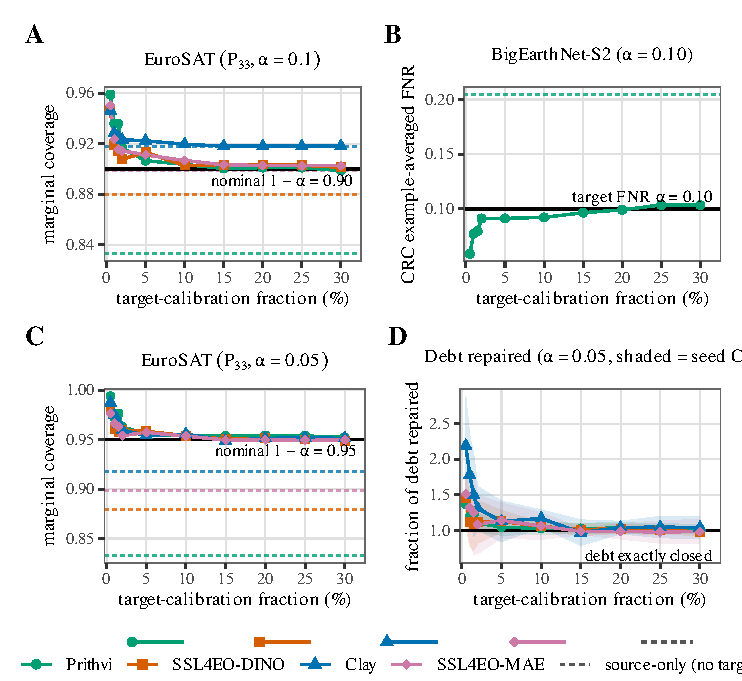
\includegraphics[width=0.95\textwidth]{F10_target_cal_planning.pdf}
\caption{Target-recalibration planning curves: annotation budget versus guarantee tightness.
\textbf{(A)}~EuroSAT-MS ($P_{33}$, $\alpha{=}0.10$): marginal coverage of the target-calibrated arm
versus the labeled fraction of the target region (\%).
\textbf{(B)}~GEO-Bench BigEarthNet-S2 ($\alpha{=}0.10$): CRC example-averaged false-negative rate
(FNR) on the same $x$-axis (Prithvi only; vacuous CRC budgets with
$\alpha < 1/(n_{\mathrm{eff}}{+}1)$ omitted).
\textbf{(C)}~EuroSAT-MS at the stricter $\alpha{=}0.05$, same coverage axes as~(A).
\textbf{(D)}~Normalized EuroSAT reading at $\alpha{=}0.05$: fraction of coverage debt repaired
versus budget (shaded bands $=$ five-seed intervals; values ${>}1$ are over-repair).
Solid coloured curves are encoders; matching dashed horizontals are budget-independent
source-only baselines (no target labels); black horizontals mark the nominal coverage
$1{-}\alpha$, target FNR $\alpha$, or exact debt clearance ($=1$ in~(D)).
The repair is not a rising ramp: wherever debt exists, the smallest usable budget already
clears the nominal level, after which curves converge onto it from the conservative side.
That shape is finite-sample conformal correction---the effective quantile
$\lceil(n{+}1)(1{-}\alpha)\rceil/n$ inflates above $1{-}\alpha$ at small $n$ (e.g.\ $0.932$ vs.\
$0.900$ at $n{=}44$, $\alpha{=}0.10$), over-covering and paying for the slack in larger sets---so
extra labels buy tightness to nominal, not validity of the guarantee.
Descriptive secondary analysis; So2Sat excluded (no local features).
}\label{fig:f10}
\end{figure*}
\FloatBarrier

Tables~\ref{tab:weighted}--\ref{tab:so2sat} are a robustness battery, not five independent findings: each
holds the frozen encoders and the coverage debt fixed and swaps exactly one variable---the correction
method (unlabeled covariate-shift reweighting in Table~\ref{tab:weighted}; label-shift-adjusted
reweighting in Table~\ref{tab:labelshift}), the source/target geographic cut (Table~\ref{tab:boundary}),
or the benchmark itself (BigEarthNet's multi-label FNR arm in Table~\ref{tab:crc}; the non-European
So2Sat benchmark in Table~\ref{tab:so2sat}). In every table the single comparison worth making is the
same one: at the shared $\alpha=0.05$ row, read the source-only (``split'') figure against the labeled
target-side repair figure in that row---the gap between them is the debt each table is stress-testing,
and it is the only number that would change the paper's claim if it closed.

% source: experiments/results/eurosat_weighted_conformal_baseline\slash results.json (alpha=0.05 coverage split/weighted/target_global and ESS frac; weighted = Tibshirani 2019 covariate-shift split conformal, density-ratio weights from a logistic src-vs-tgt discriminator on the frozen embeddings)
A stronger unlabeled baseline still does not close the debt. Is the labeled target slice truly
necessary, or would a principled unlabeled remedy suffice? As a post-hoc exploratory baseline on the
cached EuroSAT features we add covariate-shift-weighted split conformal \citep{tibshirani2019covariate}:
density-ratio weights $w(x)$ from a logistic source-vs-target discriminator on the frozen embeddings,
weighted-quantile calibration on the source scores, scored on the same shifted target
(Table~\ref{tab:weighted}). Reweighting recovers part of the debt---at $\alpha=0.05$ target coverage
rises from source-split $0.833$--$0.918$ to $0.911$--$0.938$ per encoder---but under-covers the
nominal $0.95$ for every encoder and never matches the labeled target-global arm (${\approx}0.95$).
The mechanism is visible in the weights: the effective sample size is only $0.1$--$1.6\%$ of the
calibration set --- density ratios so heavy-tailed that a handful of points dominate, a direct
signature that this real E$\to$W shift is not the pure covariate shift under which weighted conformal
is guaranteed (it also carries the class-prior shift documented in Methods). Even a principled
unlabeled correction is thus insufficient and unstable here; a small labeled target slice remains the
reliable remedy.

\begin{table*}[!t]\centering\small
\caption{Unlabeled-remedy controls on the identical EuroSAT E$\to$W split (5-seed means; full
$\alpha\in\{0.05,0.10,0.20\}$ sweep from the frozen result records): covariate-shift-weighted split
conformal (density-ratio weights from a source-vs-target discriminator on
the frozen embeddings; ``ESS'' is the weights' effective sample size as a fraction of the calibration set,
fixed before calibration and hence constant across $\alpha$) and label-shift-weighted split conformal
(Oracle: true target label marginal; BBSE: target
priors from unlabeled target predictions). Split, Weighted, ESS, and Target-global columns are from the
weighted-run record; the label-shift record reproduces Split and Target-global within $\pm0.001$. Weighted
conformal under-covers nominal at every $\alpha$ for every encoder (the ESS collapse signals the shift is
not pure covariate shift); label-shift adjustment makes three of four encoders \emph{worse} than doing
nothing, and its deficit widens at looser $\alpha$. Only the labeled target-global arm reaches
nominal.}\label{tab:weighted}\label{tab:labelshift}
\begin{tabular}{clcccccc}
\toprule
$\alpha$ & Encoder & Split & Weighted & ESS frac.\ & LS-oracle & LS-BBSE & Target-global \\
\midrule
% source: experiments/results/eurosat_weighted_conformal_baseline/results.json (split/weighted/target_global/w_ess_frac)
% source: experiments/results/labelshift_adjusted_baseline/results.json (conformal_labelshift_oracle/_bbse)
0.05 & Prithvi     & 0.833 & 0.919 & 1.6\% & 0.879 & 0.884 & 0.952 \\
0.05 & SSL4EO-DINO & 0.880 & 0.938 & 1.3\% & 0.858 & 0.867 & 0.949 \\
0.05 & SSL4EO-MAE  & 0.899 & 0.911 & 0.4\% & 0.856 & 0.865 & 0.950 \\
0.05 & Clay        & 0.918 & 0.927 & 0.1\% & 0.891 & 0.895 & 0.951 \\
\midrule
0.10 & Prithvi     & 0.833 & 0.881 & 1.6\% & 0.793 & 0.798 & 0.899 \\
0.10 & SSL4EO-DINO & 0.880 & 0.914 & 1.3\% & 0.766 & 0.774 & 0.901 \\
0.10 & SSL4EO-MAE  & 0.899 & 0.905 & 0.4\% & 0.793 & 0.803 & 0.903 \\
0.10 & Clay        & 0.918 & 0.923 & 0.1\% & 0.825 & 0.832 & 0.918 \\
\midrule
0.20 & Prithvi     & 0.833 & 0.855 & 1.6\% & 0.675 & 0.682 & 0.833 \\
0.20 & SSL4EO-DINO & 0.880 & 0.898 & 1.3\% & 0.625 & 0.639 & 0.880 \\
0.20 & SSL4EO-MAE  & 0.899 & 0.902 & 0.4\% & 0.688 & 0.704 & 0.898 \\
0.20 & Clay        & 0.918 & 0.921 & 0.1\% & 0.711 & 0.719 & 0.918 \\
\bottomrule
\end{tabular}
\end{table*}

% source: experiments/results/labelshift_adjusted_baseline/results.json (alpha=0.05 coverage: split/ls_oracle/ls_bbse/target_global; oracle+BBSE worsen 3/4 encoders; LABELSHIFT-CONTROL-VERDICT.md)
A label-shift-adjusted control rules out the class-prior confound: the $P_{33}$ cut's
severe class-prior shift (Table~\ref{tab:classprior}) raises the possibility that the
coverage debt above is a textbook label-shift effect \citep{podkopaev2021labelshift} rather than a
genuinely geographic one. We test this directly at the identical $P_{33}$ split: we reweight the
source calibration scores by $w(y)=\hat\pi_{\text{target}}(y)/\hat\pi_{\text{source}}(y)$
(Podkopaev--Ramdas label-shift-weighted split conformal), in an \emph{oracle} variant (the true
target-region label marginal, an upper bound on what prior-shift correction alone could repay) and a
deployable variant (target priors from confusion-matrix Black-Box Shift Estimation
\citep{lipton2018bbse}, using unlabeled target predictions only). Neither restores
coverage. For three of four encoders both variants make coverage worse than doing nothing
(Table~\ref{tab:labelshift}), and for Prithvi (heaviest debt) both recover only part of the gap
while remaining far below nominal and the labeled target-global arm. The overcorrection compounds at
looser risk levels---at $\alpha=0.20$ every encoder's
% source: experiments/results/labelshift_adjusted_baseline/results.json (alpha=0.20, nominal 0.80; below-nominal deficits per encoder, oracle/BBSE arms: Clay 8.9/8.1, SSL4EO-MAE 11.2/9.6, Prithvi 12.5/11.8, SSL4EO-DINO 17.5/16.1 pp; envelope 8.1--17.5 pp, all four encoders; vs the do-nothing split arm: 15.1--25.4 pp below)
label-shift-adjusted coverage sits $8.1$--$17.5$\,pp below nominal---and more than $15$\,pp below
even the do-nothing source-split arm.\footnote{The label-shift run reproduces the Split and Target-global columns of
Table~\ref{tab:weighted} within $\pm0.001$; its own covariate-shift-weighted reference column (not
shown) differs slightly because the two runs use different, both legitimate, base-rate corrections
for the density-ratio discriminator. This affects only that reference column, not the label-shift
arms.} Because label-shift weighting is
provably valid only when $P(x\mid y)$ is shift-invariant, this systematic failure rules out a pure
class-prior-shift explanation and is consistent with a within-class conditional shift in the frozen
encoders' features across regions---the geographic mechanism this paper posits, which target-side
recalibration (which assumes nothing about $P(x\mid y)$) correctly repairs and label-shift reweighting
cannot.



\begin{table*}[!t]\centering\small
\caption{Boundary-sensitivity sweep, real-shift target coverage ``split / target-global /
spatial-Mondrian'' (5-seed means; split = source-only calibration; target-global = non-spatial,
target-calibrated ablation arm; full $\alpha\in\{0.05,0.10,0.20\}$ sweep from the same frozen result
record, expanding the $\alpha{=}0.05$ headline row). $^{\dagger}$~=~Mondrian-vs-split paired CI does not
exclude $0$ (no significant restoration). At $\alpha{=}0.05$, restoration holds in $15$ of $16$
encoder$\times$boundary cells (the sole exception, Clay at $P_{50}$, where debt is ${\approx}0.014$, is
marked); at looser $\alpha$ most cells no longer need repair because shifted accuracy already approaches
nominal.}\label{tab:boundary}
\begin{tabular}{clcccc}
\toprule
$\alpha$ & Encoder & $P_{25}$ & $P_{33}$ (headline) & $P_{40}$ & $P_{50}$ \\
\midrule
% source: experiments/results/eurosat_boundary_sweep/results.json (real_shift coverage means, per fm/boundary/alpha; alpha=0.05 rows reproduce the paper's original headline row verbatim; alpha=0.10/0.20 rows expand the same frozen record; dagger = restoration.split_minus_mondrian.ci_excludes_0_positive is false)
0.05 & Prithvi & 0.792 / 0.946 / 0.952 & 0.833 / 0.952 / 0.955 & 0.843 / 0.950 / 0.955 & 0.859 / 0.949 / 0.952 \\
0.05 & SSL4EO-DINO & 0.847 / 0.947 / 0.951 & 0.880 / 0.949 / 0.956 & 0.892 / 0.950 / 0.955 & 0.896 / 0.951 / 0.955 \\
0.05 & SSL4EO-MAE & 0.865 / 0.948 / 0.957 & 0.898 / 0.950 / 0.962 & 0.910 / 0.946 / 0.962 & 0.917 / 0.952 / 0.967 \\
0.05 & Clay & 0.897 / 0.950 / 0.955 & 0.918 / 0.951 / 0.960 & 0.926 / 0.947 / 0.960 & 0.936 / 0.950 / 0.963\rlap{$^{\dagger}$} \\
\midrule
0.10 & Prithvi & 0.789 / 0.899 / 0.898 & 0.833 / 0.899 / 0.911 & 0.841 / 0.902 / 0.915 & 0.854 / 0.902 / 0.917 \\
0.10 & SSL4EO-DINO & 0.847 / 0.897 / 0.906 & 0.880 / 0.901 / 0.926\rlap{$^{\dagger}$} & 0.892 / 0.901 / 0.928\rlap{$^{\dagger}$} & 0.896 / 0.902 / 0.930\rlap{$^{\dagger}$} \\
0.10 & SSL4EO-MAE & 0.865 / 0.895 / 0.920\rlap{$^{\dagger}$} & 0.898 / 0.903 / 0.934\rlap{$^{\dagger}$} & 0.910 / 0.910 / 0.938\rlap{$^{\dagger}$} & 0.917 / 0.917 / 0.947\rlap{$^{\dagger}$} \\
0.10 & Clay & 0.897 / 0.900 / 0.920\rlap{$^{\dagger}$} & 0.918 / 0.918 / 0.936\rlap{$^{\dagger}$} & 0.926 / 0.926 / 0.935\rlap{$^{\dagger}$} & 0.936 / 0.936 / 0.943\rlap{$^{\dagger}$} \\
\midrule
0.20 & Prithvi & 0.789 / 0.802 / 0.832\rlap{$^{\dagger}$} & 0.833 / 0.833 / 0.856\rlap{$^{\dagger}$} & 0.841 / 0.841 / 0.867\rlap{$^{\dagger}$} & 0.854 / 0.854 / 0.877\rlap{$^{\dagger}$} \\
0.20 & SSL4EO-DINO & 0.847 / 0.847 / 0.850\rlap{$^{\dagger}$} & 0.880 / 0.880 / 0.888\rlap{$^{\dagger}$} & 0.892 / 0.892 / 0.896\rlap{$^{\dagger}$} & 0.896 / 0.896 / 0.902\rlap{$^{\dagger}$} \\
0.20 & SSL4EO-MAE & 0.865 / 0.865 / 0.880\rlap{$^{\dagger}$} & 0.898 / 0.898 / 0.905\rlap{$^{\dagger}$} & 0.910 / 0.910 / 0.917\rlap{$^{\dagger}$} & 0.917 / 0.917 / 0.929\rlap{$^{\dagger}$} \\
0.20 & Clay & 0.897 / 0.897 / 0.897\rlap{$^{\dagger}$} & 0.918 / 0.918 / 0.918\rlap{$^{\dagger}$} & 0.926 / 0.926 / 0.926\rlap{$^{\dagger}$} & 0.936 / 0.936 / 0.936\rlap{$^{\dagger}$} \\
\bottomrule
\end{tabular}
\end{table*}

\subsection{Replication on a second benchmark (BigEarthNet)}
We replicate the phenomenon on a second real EO benchmark: GEO-Bench \citep{lacoste2023geobench} \texttt{m-bigearthnet}
(BigEarthNet-S2 \citep{sumbul2019bigearthnet}; 7{,}669 usable tiles, real lat/lon, $36.96$--$67.80^\circ$N). We apply two complementary
analyses.

% source: experiments/results/bigearthnet_coverage_debt.json (ece 0.36->0.56 prithvi, 0.15->0.42 ssl4eo, 0.33->0.59 clay; acc in 0.50-0.61, shift 0.27-0.37)
A documented dominant-label single-label proxy (12 classes, $\ge60$ tiles each)
lets the single-label LAC harness apply unchanged. All three frozen FMs replicate the pattern: ECE degrades
($0.36\to0.56$ Prithvi, $0.15\to0.42$ SSL4EO, $0.33\to0.59$ Clay) and spatial-Mondrian restores coverage
to near-nominal at all three risk levels (Fig.~\ref{fig:f5}). The proxy is a hard task (frozen-probe accuracy $0.50$--$0.61$
in-distribution, dropping to $0.27$--$0.37$ under shift), so restoration is bought at large prediction-set
sizes (${\sim}6$--$10$ of $12$ classes)---a coarse, qualitative replication.

% source: experiments/results/bigearthnet_perlabel_conformal.json (alpha=0.10, 3-FM means: in 0.925, shift 0.752, mondrian 0.908, mean per-label debt 0.173, mondrian set size 20.9; per-seed across-label CIs exclude 0 at 0.10/0.20 for all FMs)
We extend the analysis with rigorous per-class binary conformal
prediction on the 43-class multi-hot labels. For each of 39 well-populated labels ($\ge120$ global
positives; 27 active per seed after per-split filtering), we fit an independent binary probe
(StandardScaler, L2-logistic, $C=1$, 5~seeds) on source-region embeddings and calibrate per-label
recall-coverage $\Pr(c\in\mathcal{C}(x)\mid y_c=1)$ via source-only split-conformal and target-side
spatial-Mondrian arms. The coverage-debt phenomenon replicates per-label: mean recall-coverage drops from
0.92 in-distribution to 0.75 under shift ($\alpha=0.10$; mean per-label debt
0.173), with spatial-Mondrian restoring to 0.91 (per-label paired CI excludes $0$ at
$\alpha\in\{0.10,0.20\}$ for all three FMs; Fig.~\ref{fig:f6}). Predicted-label set sizes remain large
(20.9 of 27 active labels per tile at $\alpha=0.10$), reflecting the geographic
distributional mismatch and the recall requirement. Per-label conformal is more principled than the
dominant-label proxy---it offers independent per-class recall guarantees---but both yield comparably large
prediction sets under this hard pan-European shift.

% source: experiments/results/bigearthnet_crc_arm-exec-2026-06-29.json (n=5 box run 2026-07-14; bootstrap fnr_in_crc 0.105 prithvi, fnr_sh_crc 0.206-0.277 at alpha=0.10; fnr_sh_mond <= nominal; set sizes ss_sh_crc/ss_sh_mond; gate overall_verdict SUCCESS, all 5 encoders story holds)
This conformal-risk-control (CRC) arm, which gives a finite-sample FNR guarantee, is the substrate for the
paper's primary decoupling result (Table~\ref{tab:fnrdecouple}); here we give its full per-$\alpha$
calibration and repair numbers for all five frozen encoders. Per-label split-conformal offers per-class
recall calibration but no finite-sample guarantee on the example-averaged false-negative rate (FNR). We
therefore add a conformal-risk-control (CRC) arm \citep{angelopoulos2024crc} on the same frozen-feature caches, splits,
$4\times4$ Mondrian grid, and per-label probes (per-example FNR loss, monotone in the threshold $\lambda$;
exact weighted-quantile calibration; 5 seeds; percentile-bootstrap CIs, $B{=}2000$). The three-step story
repeats under the marginal-FNR guarantee for every encoder (Table~\ref{tab:crc}): (i) source-calibrated CRC meets the
target FNR in-distribution (e.g.\ $0.105$ at $\alpha{=}0.10$, Prithvi); (ii) the same $\widehat{\lambda}$ incurs
FNR debt under the geographic shift ($2$--$4\times$ the nominal level, e.g.\ $0.206$--$0.277$ at
$\alpha{=}0.10$); (iii) a Mondrian-CRC arm calibrated per spatial bin on the target-region slice restores
marginal FNR to at-or-below nominal, at the cost of larger label sets (${\sim}17$--$18$ vs.\
${\sim}8$--$12$ labels/tile at $\alpha{=}0.10$). An honest efficiency note: CRC controls only the
example-averaged FNR, so its in-distribution sets are smaller than per-label split-conformal's, and
in-distribution FNR at $\alpha{=}0.05$ fluctuates slightly above nominal (mean $0.052$--$0.056$), consistent
with the expectation-level $\mathbb{E}[L]\le\alpha$ guarantee---which holds in expectation over calibration
draws, not per individual run, so a single run landing marginally above $\alpha$ is expected, not a violation. Like spatial-Mondrian conformal, Mondrian-CRC
requires labeled target-region calibration data---a shift-aware remedy, not a free lunch.
The CRC / method comparison is summarized in Fig.~\ref{fig:crcfnr}.

\begin{table*}[htbp]\centering\small
\caption{CRC arm on GEO-Bench \texttt{m-bigearthnet} (marginal per-example FNR; mean [95\% bootstrap CI]
pooled over 5 seeds). Source-calibrated CRC meets nominal in-distribution, incurs FNR debt under the real
E$\to$W shift, and target-side Mondrian-CRC restores it. Set sizes are labels/tile (of ${\sim}27$ active)
under shift.}\label{tab:crc}
\begin{tabular}{clcccc}
\toprule
$\alpha$ & Encoder & CRC FNR in-dist & CRC FNR shift & Mondrian-CRC FNR shift & Sets CRC/Mond. \\
\midrule
% source: experiments/results/bigearthnet_crc_arm-exec-2026-06-29.json (n=5 box run 2026-07-14; bootstrap blocks per fm/alpha; folded from box_pulled_2026-07-14, backup .bak-n3)
0.05 & Prithvi & 0.055 [0.051,0.058] & 0.130 [0.125,0.135] & 0.031 [0.029,0.034] & 15.5 / 22.3 \\
0.05 & Clay & 0.053 [0.049,0.056] & 0.176 [0.171,0.182] & 0.022 [0.020,0.024] & 13.3 / 23.8 \\
0.05 & SSL4EO-DINO & 0.053 [0.050,0.057] & 0.191 [0.185,0.196] & 0.032 [0.029,0.034] & 10.6 / 22.3 \\
0.05 & SSL4EO-MAE & 0.052 [0.048,0.055] & 0.170 [0.164,0.175] & 0.030 [0.028,0.033] & 11.8 / 22.1 \\
0.05 & DOFA & 0.056 [0.052,0.059] & 0.169 [0.164,0.175] & 0.021 [0.019,0.024] & 13.0 / 24.1 \\
\midrule
0.10 & Prithvi & 0.105 [0.101,0.110] & 0.206 [0.200,0.212] & 0.083 [0.079,0.086] & 11.9 / 18.2 \\
0.10 & Clay & 0.108 [0.103,0.113] & 0.277 [0.271,0.283] & 0.082 [0.078,0.086] & 9.7 / 18.2 \\
0.10 & SSL4EO-DINO & 0.107 [0.102,0.112] & 0.277 [0.271,0.283] & 0.082 [0.078,0.086] & 7.9 / 17.4 \\
0.10 & SSL4EO-MAE & 0.108 [0.103,0.113] & 0.262 [0.256,0.268] & 0.084 [0.080,0.088] & 8.6 / 17.1 \\
0.10 & DOFA & 0.107 [0.103,0.112] & 0.249 [0.243,0.256] & 0.080 [0.076,0.084] & 9.9 / 18.1 \\
\midrule
0.20 & Prithvi & 0.205 [0.199,0.211] & 0.346 [0.339,0.353] & 0.184 [0.179,0.190] & 8.0 / 12.9 \\
0.20 & Clay & 0.203 [0.197,0.209] & 0.426 [0.419,0.433] & 0.185 [0.179,0.190] & 6.4 / 12.9 \\
0.20 & SSL4EO-DINO & 0.206 [0.200,0.212] & 0.401 [0.394,0.408] & 0.191 [0.185,0.197] & 5.3 / 11.1 \\
0.20 & SSL4EO-MAE & 0.209 [0.202,0.215] & 0.408 [0.401,0.415] & 0.189 [0.184,0.195] & 5.5 / 11.3 \\
0.20 & DOFA & 0.203 [0.196,0.209] & 0.384 [0.377,0.391] & 0.187 [0.181,0.193] & 6.7 / 12.4 \\
\bottomrule
\end{tabular}
\end{table*}

\begin{figure*}[htbp]\centering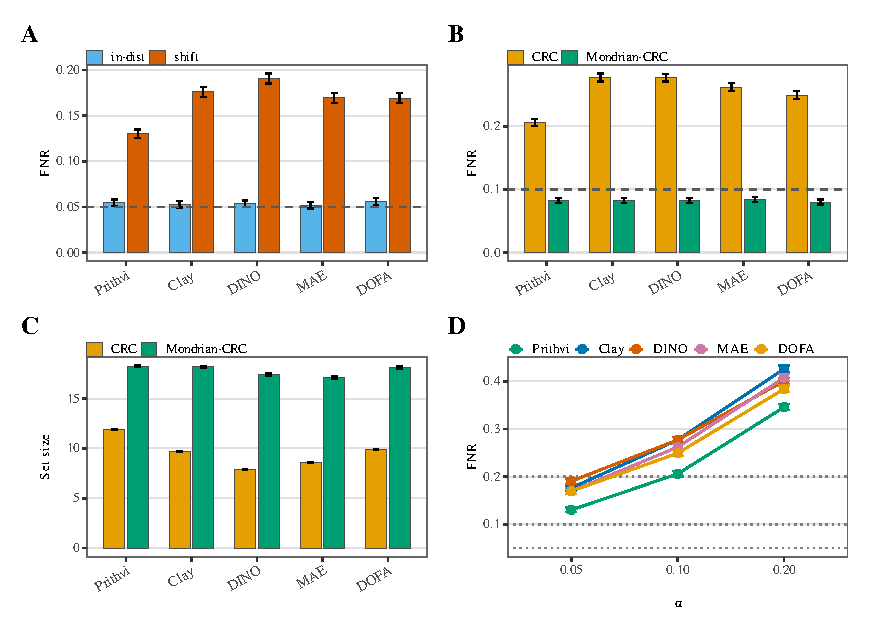
\includegraphics[width=0.95\textwidth]{F13_crc_fnr.pdf}
\caption{CRC on BigEarthNet (frozen multi-seed bootstrap means with 95\% CIs; no new runs).
All panels use example-averaged FNR (or set size) pooled over five seeds; error bars are percentile bootstrap 95\% intervals ($B{=}2000$).
Encoder ticks and the (D) colour key abbreviate SSL4EO-DINO/MAE as DINO/MAE (Prithvi, Clay, DINO, MAE, DOFA).
(A)~Source-calibrated CRC FNR in-distribution vs.\ under the E$\to$W geographic shift at $\alpha{=}0.05$ (blue $=$ in-dist, vermillion $=$ shift; dashed $=$ nominal FNR level $\alpha$). In-distribution meets the risk level; the same $\widehat{\lambda}$ incurs large FNR debt under shift.
(B)~Shift FNR at $\alpha{=}0.10$: source-calibrated CRC vs.\ target-side Mondrian-CRC (orange $=$ CRC, green $=$ Mondrian-CRC; dashed $=$ nominal $\alpha$). Mondrian-CRC restores FNR to at-or-below nominal for every encoder.
(C)~Mean set-size cost under shift at the same $\alpha{=}0.10$ (labels/tile of ${\sim}27$ active): Mondrian-CRC's restore comes with larger sets than source-calibrated CRC (shared orange/green method colours with (B)).
(D)~Source-calibrated CRC FNR under shift across $\alpha\in\{0.05,0.10,0.20\}$ by encoder (coloured lines; dotted horizontals $=$ nominal $\alpha$ at each risk level).
}\label{fig:crcfnr}\end{figure*}
\FloatBarrier

\subsection{External validation on a non-European benchmark (GEO-Bench m-so2sat)}
Both benchmarks above are European Sentinel-2. To test whether the coverage-debt phenomenon and its
target-side repair survive outside Europe, we repeat the harness on GEO-Bench \citep{lacoste2023geobench}
\texttt{m-so2sat} (So2Sat LCZ42 \citep{zhu2020so2sat}; 42 cities across multiple continents; 17 local-climate-zone classes),
using GEO-Bench's own train/valid (source) vs.\ held-out test-city (target) partition as the shift. Because
this release ships no per-tile latitude/longitude in our repo, there is no spatial-Mondrian arm here;
we compare only source-only split-conformal against a non-spatial, target-calibrated arm
(\emph{target-global}), i.e.\ exactly the label-access ablation that Table~\ref{tab:boundary} isolated as the
active ingredient on EuroSAT. All five frozen encoders now complete (Prithvi, Clay, SSL4EO ViT-S/16 MAE
% source: experiments/results/so2sat_coverage_debt/results.json (n=5 box run 2026-07-14; blocked_fms={}, Clay v1.5 now loaded; backup .bak-n2)
native-S2, SSL4EO-MAE ViT-B/16, DOFA); the earlier Clay v1.5 checkpoint-load failure ($>4$\,GB expected in
cache) was resolved on the extraction host, so the encoder-ranking diagnostic is now available on this
benchmark too (all five extracted on the hash-gated frozen substrate).

% source: experiments/results/so2sat_coverage_debt/results.json (n=5: acc in->shift 0.670->0.522 prithvi, 0.713->0.569 clay, 0.781->0.601 ssl4eo, 0.796->0.637 ssl4eo_mae, 0.777->0.608 dofa; alpha 0.05 split cov 0.877-0.904, target_global 0.950-0.963; restoration CI excludes 0 in all 15 debt cells)
The debt-and-repair pattern replicates outside Europe: under the held-out-city shift, accuracy
drops by ${\approx}0.14$--$0.18$ across the five encoders ($0.670\to0.522$ Prithvi up to $0.796\to0.637$
SSL4EO-MAE)---a genuine, non-trivial distribution shift.
Source-only split-conformal under-covers at every risk level and every encoder ($\alpha=0.05$: $0.877$--$0.904$;
$\alpha=0.20$: $0.632$--$0.685$), and the non-spatial target-calibrated arm restores coverage to
near-nominal ($\alpha=0.05$: $0.950$--$0.963$), with the paired-seed restoration CI
excluding $0$ in every one of the fifteen debt cells ($5$ encoders ${\times}\,3$ risk levels; Table~\ref{tab:so2sat}). Restoration is bought at modest set sizes
(${\sim}2$--$6$ of $17$ classes), not vacuous full-label sets. This external label-access
replication now spans all five encoders on a non-European, multi-continent benchmark: it confirms the operative part of the
finding---\emph{target-side conformal recalibration}, not spatial binning, repays the debt. It still lacks a
spatial-Mondrian arm (no per-tile lat/lon), so it tests the label-access mechanism only; but with all
five encoders now loadable it also carries the per-class conditional-coverage diagnostic (below). A data-provenance note applies: \texttt{m-so2sat} was
obtained via GEO-Bench~1.0 (HuggingFace \texttt{recursix/geo-bench-1.0}) after the designed v0.9.1 Zenodo
pull was unreachable, with a label map reconstructed from per-sample ground truth (21{,}964/21{,}964
samples, $0$ failures); the v0.9.1$\to$v1.0 content differences were not independently audited
(see the data-provenance note in the code archive).

\begin{table*}[!t]\centering\small
\caption{Non-European external validation on GEO-Bench \texttt{m-so2sat} (17 local-climate-zone classes,
42 multi-continent cities; 5-seed means). Target coverage ``split / target-global'' under the held-out-city
shift (split = source-only calibration; target-global = non-spatial, target-calibrated label-access arm; no
spatial-Mondrian arm, as this release carries no per-tile lat/lon in our repo). Set sizes (of 17 classes) in
brackets. All five encoders now load (Clay v1.5 checkpoint-load failure resolved).}\label{tab:so2sat}
\begin{tabular}{clccc}
\toprule
$\alpha$ & Encoder & Split [set] & Target-global [set] & Acc.\ in$\to$shift \\
\midrule
% source: experiments/results/so2sat_coverage_debt/results.json (n=5 box run 2026-07-14; cells means)
0.05 & Prithvi & 0.904 [3.92] & 0.956 [5.72] & 0.670$\to$0.522 \\
0.05 & Clay & 0.891 [3.32] & 0.954 [5.08] & 0.713$\to$0.569 \\
0.05 & SSL4EO ViT-S/16 MAE & 0.880 [2.42] & 0.962 [4.25] & 0.781$\to$0.601 \\
0.05 & SSL4EO-MAE ViT-B/16 & 0.882 [2.18] & 0.950 [3.47] & 0.796$\to$0.637 \\
0.05 & DOFA & 0.877 [2.49] & 0.963 [5.35] & 0.777$\to$0.608 \\
\midrule
0.10 & Prithvi & 0.825 [2.71] & 0.907 [4.02] & 0.670$\to$0.522 \\
0.10 & Clay & 0.808 [2.27] & 0.888 [3.24] & 0.713$\to$0.569 \\
0.10 & SSL4EO ViT-S/16 MAE & 0.775 [1.67] & 0.904 [2.75] & 0.781$\to$0.601 \\
0.10 & SSL4EO-MAE ViT-B/16 & 0.795 [1.57] & 0.896 [2.38] & 0.796$\to$0.637 \\
0.10 & DOFA & 0.781 [1.69] & 0.918 [3.30] & 0.777$\to$0.608 \\
\midrule
0.20 & Prithvi & 0.685 [1.62] & 0.819 [2.65] & 0.670$\to$0.522 \\
0.20 & Clay & 0.672 [1.39] & 0.795 [2.17] & 0.713$\to$0.569 \\
0.20 & SSL4EO ViT-S/16 MAE & 0.632 [1.08] & 0.809 [1.88] & 0.781$\to$0.601 \\
0.20 & SSL4EO-MAE ViT-B/16 & 0.654 [1.04] & 0.793 [1.59] & 0.796$\to$0.637 \\
0.20 & DOFA & 0.634 [1.07] & 0.823 [1.99] & 0.777$\to$0.608 \\
\bottomrule
\end{tabular}
\end{table*}

% source: so2sat_roster_stage_2026-07-13/perclass_conditional_summary.json (alpha=0.05, conformal_split arm, 5 seeds;
%   worst_class_cov vs accuracy rho=-0.10 p=0.87 5 inversions; vs shift-ECE rho=+0.60 p=0.285 3 inversions; both not recoverable)
As a second, multiclass conditional-coverage dissociation, with all five encoders loadable, m-so2sat
also lets us re-run the per-class conditional-coverage diagnostic of the EuroSAT conditional finding
(\S\ref{sec:results}) on a second, $17$-class multiclass benchmark. At $\alpha{=}0.05$ we measure, for the
source-only split predictor, the worst individual LCZ class coverage per encoder (Table~\ref{tab:so2satcond}).
It dissociates from both shifted accuracy and shift-ECE:
$\mathrm{Spearman}(\text{worst-class cov},\text{acc})=-0.10$ ($p{=}0.87$, $5$ pairwise inversions) and
$\mathrm{Spearman}(\text{worst-class cov},\text{ECE}_{\mathrm{sh}})=+0.60$ ($p{=}0.29$, $3$ inversions);
the class-coverage spread scrambles likewise ($\rho=-0.30$ against each, $6$ inversions). The most accurate
encoder here (SSL4EO-MAE, acc $0.637$) is not the one that best protects its worst class, and the
worst-covered class ($0.689$--$0.733$ across encoders, under marginal coverage $0.877$--$0.904$) is
under-served regardless of accuracy or calibration ranking. This corroborates the EuroSAT
conditional-coverage finding with an independent multiclass benchmark---though on the unrepaired
split sets here (no target-side repair or spatial arm on this release), and, like the EuroSAT case, it is
post-hoc, exploratory, and small-$n$ ($n{=}5$, all $p>0.28$; \S\ref{sec:limitations}).

\begin{table*}[!t]\centering\small
\caption{Per-class conditional coverage on GEO-Bench \texttt{m-so2sat} ($17$ LCZ classes; source-only
split-conformal, $\alpha{=}0.05$; 5 seeds). The worst individual-class coverage dissociates from shifted
accuracy and shift-ECE ($\mathrm{Spearman}=-0.10/+0.60$; $5/3$ pairwise inversions), a second
multiclass instance of the EuroSAT conditional-coverage collapse.}\label{tab:so2satcond}
\begin{tabular}{lccccc}
\toprule
Encoder & Acc.\ shift & ECE shift & Marg.\ cov & Worst-class cov & Class spread \\
\midrule
% source: so2sat_roster_stage_2026-07-13/perclass_conditional_summary.json (per_encoder, alpha 0.05, split arm)
Prithvi             & 0.522 & 0.364 & 0.904 & 0.731 & 0.269 \\
Clay                & 0.569 & 0.325 & 0.891 & 0.732 & 0.264 \\
SSL4EO ViT-S/16 MAE & 0.601 & 0.114 & 0.880 & 0.689 & 0.302 \\
SSL4EO-MAE ViT-B/16 & 0.637 & 0.173 & 0.882 & 0.702 & 0.269 \\
DOFA                & 0.608 & 0.214 & 0.877 & 0.733 & 0.253 \\
\bottomrule
\end{tabular}
\end{table*}

% Figures: all regenerated from result JSONs by figures/p3_figs.R, figures/p3_bigearthnet.R,
% figures/p3_bigearthnet_perlabel.R (make figures). Local copies live in ./figures/.
% source (F1-F3): experiments/results/eurosat_stage2_multifm_multialpha/results_fivefm_figures_2026-07-13.json
%   = deep-merged figure input: four battery encoders from the PROTECTED canonical results.json
%   (byte-equivalent) + the corrected DOFA fifth-encoder block (forward_features 768-d, re-run 2026-07-13,
%   from eurosat_stage2_dofa_corrected_2026-07-13/results.json). Canonical results.json is never modified.
% F1/F2/F3/F5/F6 promoted from single-column `figure` (width relative to \columnwidth)
% to double-column-spanning `figure*` (width relative to \textwidth): a single-column
% width in this venue is too narrow for the shared canonical-sized PDFs to clear the
% 7pt-effective floor (typography re-audit, 2026-07-16; content/data unchanged, layout only).
% G004 (2026-08-12): F1--F3 refreshed to four-panel PDFs + ISPRS captions; F8--F14 ported.
\begin{figure*}[htbp]\centering
\includegraphics[width=0.95\textwidth]{F1_debt_vs_robustness.pdf}
\caption{Four-panel coverage-debt diagnostic across five frozen encoders (shared colour legend:
Clay, SSL4EO-MAE, SSL4EO-DINO, DOFA, Prithvi).
(A)~Mean in-shift ECE (coverage debt) vs.\ the number of risk levels
$\alpha\in\{0.05,0.10,0.20\}$ where spatial-Mondrian \emph{restores} target coverage---i.e.\ the
paired gap CI excludes~$0$ in the positive direction. Debt orders
Prithvi $>$ DOFA $>$ SSL4EO-DINO $>$ SSL4EO-MAE $>$ Clay; repair counts are weakly monotone
(Prithvi $=$ DOFA~$2$, others~$1$).
(B)~Shifted top-1 accuracy vs.\ $\alpha$ (flat across risk levels; ranking matches debt).
(C)~Boundary-sweep check on the four battery encoders (DOFA absent from that frozen sweep):
\#$\alpha$ restored at spatial cuts P25--P50.
(D)~So2Sat LCZ cross-continent label-access check: source-split vs.\ target-global coverage
(facets); dashed horizontal guides mark nominal $1-\alpha$ at each $\alpha$ (not error bars);
vertical whiskers are seed-level CIs.
Set-size cost of the same repair appears in the companion four-panel set-size figure.}\label{fig:f1}\end{figure*}

\begin{figure*}[htbp]\centering
\includegraphics[width=0.95\textwidth]{F2_coverage_restoration.pdf}
\caption{Coverage restoration under real geographic shift (error bars = seed-level $t$-CIs, $n{=}5$;
dashed = nominal $1-\alpha$).
(a)~EuroSAT $P_{33}$: source split-conformal vs.\ spatial-Mondrian coverage by encoder and $\alpha$
(five encoders, including DOFA).
(b)~Same split vs.\ Mondrian contrast at non-$P_{33}$ spatial cuts (P25/P40/P50); row = arm,
colour = encoder (four-encoder battery; DOFA absent from this frozen record).
(c)~Five conformal arms at $\alpha{=}0.10$ (ticks: split, tgt-glob, Mondrian, weighted, class-Mond).
(d)~Label-shift controls at $\alpha{=}0.10$ (ticks: split, tgt-glob, wtd-cov, LS-oracle, LS-BBSE).
Spatial-Mondrian restores where debt exists; DOFA's shifted split coverage is $0.851$ at every $\alpha$
and spatial-Mondrian lifts it to $0.951/0.913/0.873$.}\label{fig:f2}\end{figure*}

\begin{figure*}[htbp]\centering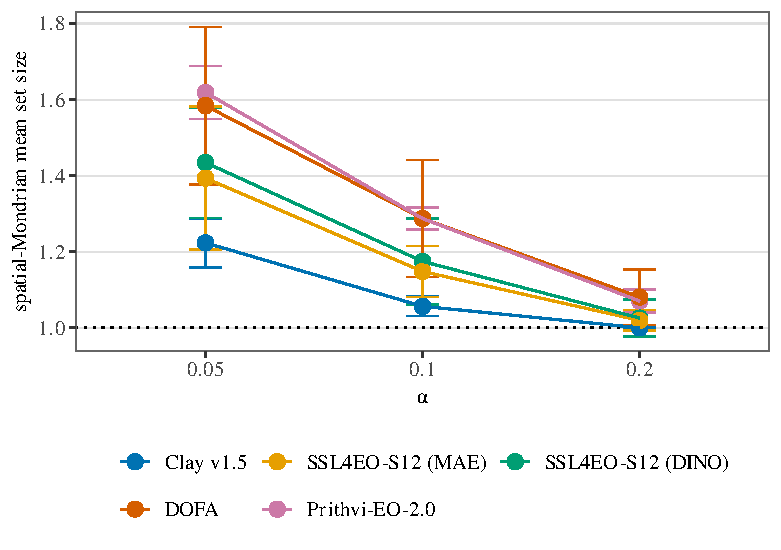
\includegraphics[width=0.95\textwidth]{F3_setsize_vs_alpha.pdf}
\caption{Four-panel set-size cost of restoration (error bars seed-level $t$-CIs, $n{=}5$; dotted line $=$
singleton floor of set size~$1$). Shared encoder colours throughout; panel~(c) uses
linetype/shape for split vs.\ spatial-Mondrian.
(a)~EuroSAT spatial-Mondrian mean set size vs.\ $\alpha$ (rises above the floor only where
Mondrian repays coverage debt; DOFA $1.58/1.29/1.08$ at $\alpha=0.05/0.10/0.20$). (b)~Source
split-conformal set size on the \emph{same} $y$-scale as~(a): every encoder sits on the singleton floor
($\approx1.000$), so the excess size in~(a) is the restoration cost. (c)~Set size vs.\ spatial boundary
percentile at $\alpha{=}0.10$ (solid $=$ source split; dashed $=$ spatial-Mondrian). (d)~So2Sat LCZ
(17~classes) source-split vs.\ target-global set size in side-by-side facets---larger absolute sets than
EuroSAT, on its own $y$-scale.}\label{fig:f3}\end{figure*}
\FloatBarrier

% Figure numbering intentionally skips Figure 4: the former F4 (set-size-vs-alpha panel) was consolidated
% into Fig.~\ref{fig:f3}; no reference to a Figure 4 remains in the text. Left as a note for maintainers.
\begin{figure*}[htbp]\centering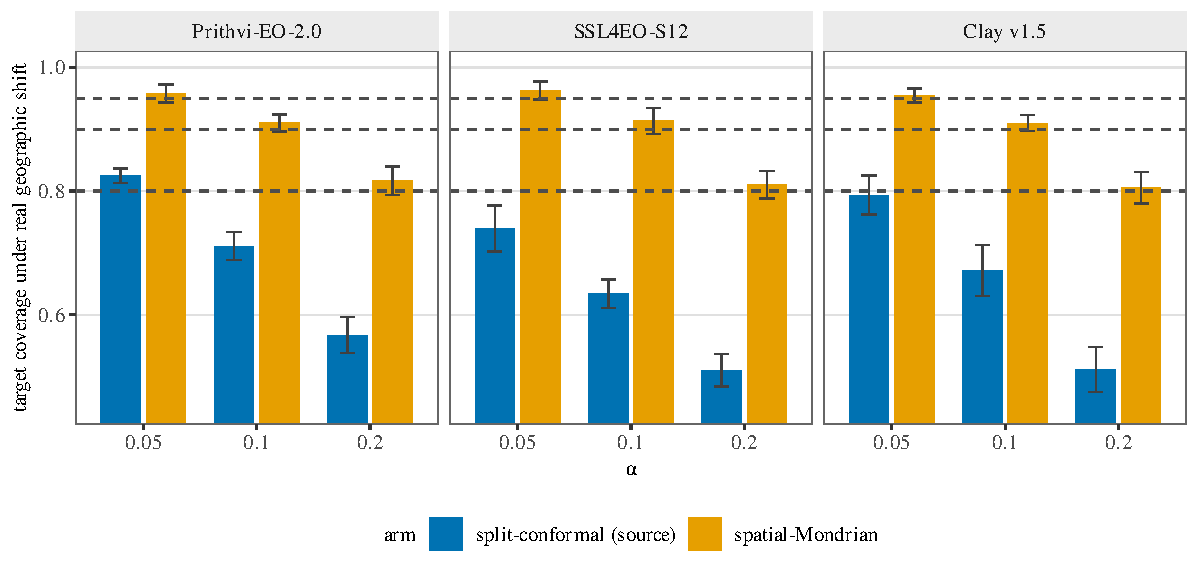
\includegraphics[width=0.95\textwidth]{F5_bigearthnet_domlabel.pdf}
\caption{Dominant-label proxy on GEO-Bench \texttt{m-bigearthnet}: multi-hot BigEarthNet-S2 tiles
reduced to the most frequent of 12 well-populated classes under a real geographic E$\to$W shift
(single-label LAC harness unchanged). Columns are the three frozen encoders (Prithvi-EO-2.0,
SSL4EO-S12, Clay~v1.5). Within each panel, blue bars are source-only split-conformal and orange bars
are target-side spatial-Mondrian at $\alpha\in\{0.05,0.10,0.20\}$. Short black dashed segments mark
the nominal coverage level $1-\alpha$ at each $\alpha$ (legend: ``nominal $1-\alpha$''); vertical
whiskers on the bars are seed-level Student~$t$ intervals ($n{=}5$), not the same mark. Coverage debt
and Mondrian restoration replicate across all three encoders. This proxy is a coarse, qualitative
replication; the companion per-label multi-label analysis is the primary BigEarthNet evidence.}\label{fig:f5}\end{figure*}

\begin{figure*}[htbp]\centering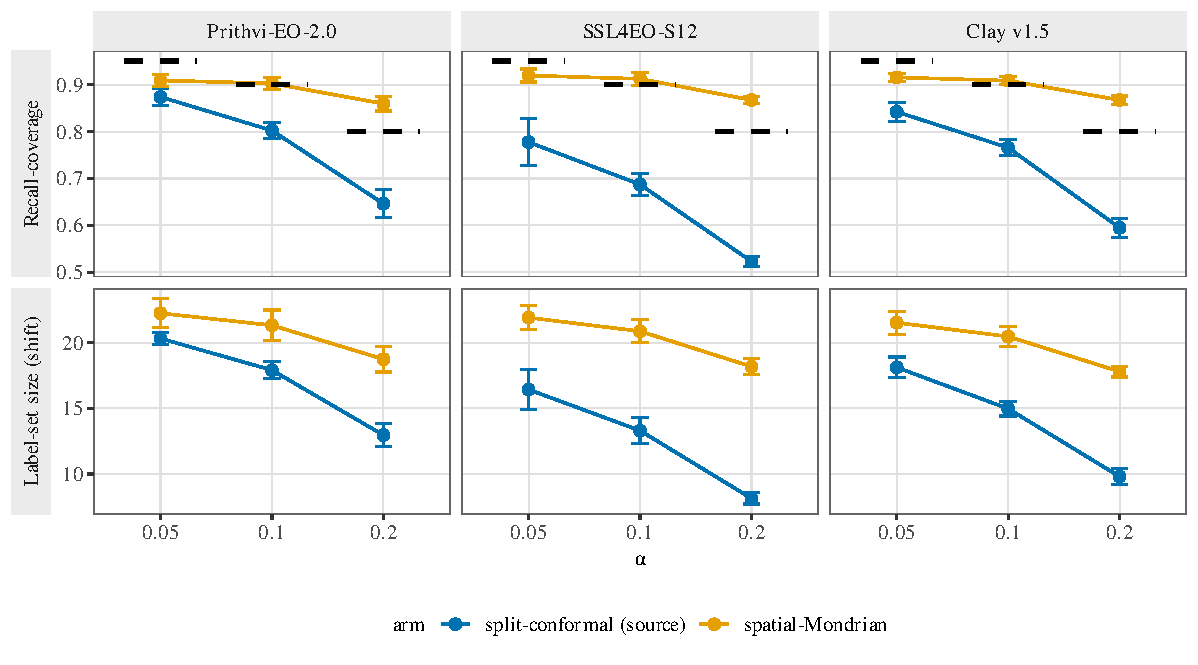
\includegraphics[width=0.95\textwidth]{F6_bigearthnet_perlabel.pdf}
\caption{Per-label multi-label conformal on GEO-Bench \texttt{m-bigearthnet}
(BigEarthNet-S2; 27 active labels after per-split filtering; real geographic E$\to$W shift).
Columns are frozen encoders; rows are (top) mean per-label recall-coverage
$\Pr(c\in\mathcal{C}(x)\mid y_c=1)$ and (bottom) mean predicted
label-set size per tile. Blue = source-only split-conformal; orange = target-side spatial-Mondrian;
$\alpha\in\{0.05,0.10,0.20\}$. Short black dashed segments in the top row are nominal $1-\alpha$
guides (legend: ``nominal $1-\alpha$''), not error bars; vertical whiskers on the points are
seed-level Student~$t$ intervals ($n{=}5$). Mondrian restores per-label coverage at
$\alpha\in\{0.10,0.20\}$ (paired CI across labels excludes~$0$) for all three FMs. Relative to the
dominant-label proxy, this per-label analysis is primary: it supplies independent per-class recall
guarantees rather than a single-label reduction.}\label{fig:f6}\end{figure*}
\FloatBarrier

\section{Discussion}\label{sec:discussion}

\subsection{Interpretation}
A conformal audit of a frozen GFM earns its keep where accuracy and calibration go silent
\citep{guo2017calibration,ovadia2019uncertainty}. On multi-label FNR risk control, every one of
thirteen frozen encoders incurs a geographic FNR debt under shift ($2.6$--$4.7\times$ nominal) that
only a labeled target slice repairs; accuracy does not reliably identify the most robust
encoder---the least accurate is the most robust, yet at $n{=}13$ the rank correlation is only a weak
positive ($\rho{=}+0.32$; Table~\ref{tab:fnrdecouple}). On per-class conditional coverage, restoring the
marginal guarantee can still leave one land-cover class covered at $0.850$ under a $0.956$ marginal
(Table~\ref{tab:condcov}), again unpredictable from the scalars a practitioner would rank on.
Symmetrically, the audit adds little in the high-accuracy singleton regime: marginal set size is then a
deterministic restatement of accuracy, so EuroSAT at full data is a mapped negative control rather than
a decoupling, and the preregistered efficiency-decoupling route is falsified. Within that boundary, the
descriptive coverage-debt ranking remains useful---ordering Prithvi, SSL4EO-DINO, SSL4EO-MAE, and Clay
consistently across risk levels---but we avoid a ``universal fix'' claim: where shifted accuracy already
meets the nominal level, there is no debt and no repair. Relative to accuracy-centric GFM surveys and
benchmarks \citep{xiao2025rsfm,lacoste2023geobench,ghamisi2025sustainfm}, the increment is pricing
geographic coverage debt rather than OOD accuracy alone.

\subsection{Mechanisms and controls}
Headline coverage and ranking numbers use an unadjusted logistic probe and therefore inherit the
$P_{33}$ source/target class-prior mismatch (Methods; up to $6.54\times$ enrichment / $\sim\!4.7\times$
depletion for individual EuroSAT classes; Fig.~\ref{fig:classprior}).


\begin{table*}[htbp]\centering\small
\caption{EuroSAT-MS per-class frequency at the $P_{33}$ longitude cut (source = E/Central Europe,
$n{=}18{,}090$; target = W/Iberian-Atlantic Europe, $n{=}8{,}910$). Classes not listed shift by
${<}2.4\times$.}\label{tab:classprior}
\begin{tabular}{lccc}
\toprule
Class & Source \% & Target \% & Target/Source ratio \\
\midrule
% source: experiments/results/eurosat_stage2_multifm_multialpha/recompute_class_prior_balanced_control_2026-07-01.json (class_prior_shift_at_P33)
5 (Pasture) & 2.62 & 17.13 & $6.54\times$ (enriched) \\
2 (HerbaceousVegetation) & 7.68 & 18.07 & $2.35\times$ (enriched) \\
9 (SeaLake) & 14.10 & 5.04 & $0.36\times$ (depleted) \\
8 (River) & 11.60 & 4.51 & $0.39\times$ (depleted) \\
1 (Forest) & 15.02 & 3.16 & $0.21\times$ ($\sim\!4.7\times$ depleted) \\
\bottomrule
\end{tabular}
\end{table*}

\begin{figure*}[htbp]\centering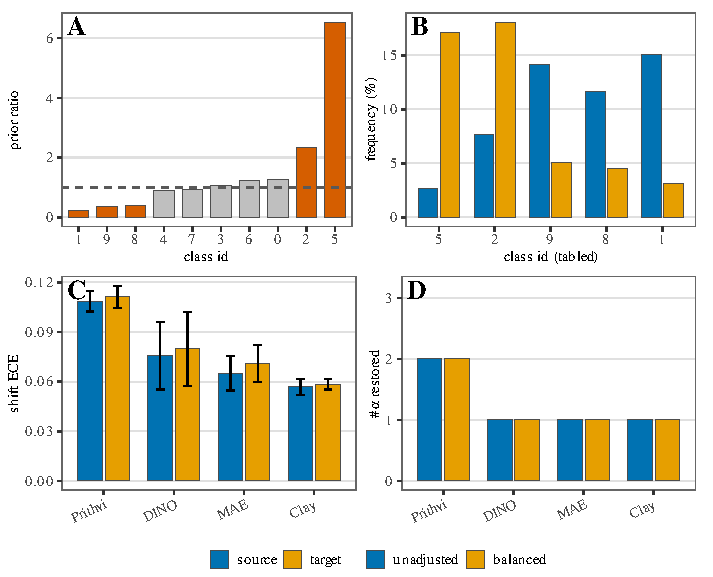
\includegraphics[width=0.95\textwidth]{F14_classprior.pdf}
\caption{Class-prior / balanced-probe control at the frozen $P_{33}$ cut (no new runs).
\textbf{A:}~target/source class-prior ratio by EuroSAT class id (orange~=~five extreme classes;
grey~=~others); dashed line at ratio~$1$ (no prior shift).
\textbf{B:}~source vs.\ target class frequency (\%) for those five classes.
\textbf{C:}~shift ECE at $\alpha{=}0.05$ under the unadjusted (headline) vs.\ class-balanced probe;
error bars are 5-seed $t$-CIs.
\textbf{D:}~count of $\alpha\in\{0.05,0.10,0.20\}$ at which spatial-Mondrian restores coverage
(paired restoration CI excludes~$0$)---the ``\#$\alpha$ repaired'' count, not Mondrian
coverage itself.
Shared bottom legend: frequency (B)~=~source/target; probe (C--D)~=~unadjusted/balanced
(same blue/orange hues, distinct meanings).
Principle: the balanced probe is a \emph{control}---encoder ranking by shift-ECE and repair counts
should be stable if the $P_{33}$ class-prior mismatch is not driving the finding.}
\label{fig:classprior}\end{figure*}
\FloatBarrier

\begin{table*}[htbp]\centering\small
\caption{Class-prior-shift control: class-balanced sample weighting vs.\ the paper's unadjusted logistic
probe, re-fit on the identical cached frozen embeddings (no GPU re-extraction), 5 seeds, real E$\to$W
shift. Top panel (EuroSAT, $\alpha=0.05$): ECE-shift ranking and per-encoder repair count (of 3
$\alpha$'s) are unchanged under the balanced control. Bottom panel (BigEarthNet-S2, $\alpha=0.10$,
per-label conformal): the analogous balanced-probe refit of the per-label harness (previously reported
only in prose) leaves mean per-label debt and Mondrian restoration essentially unchanged for all three
available FMs (SSL4EO-MAE was not run in the per-label BigEarthNet harness).}\label{tab:balanced}
\begin{tabular}{lcccccc}
\toprule
& \multicolumn{3}{c}{Unadjusted (paper headline)} & \multicolumn{3}{c}{Balanced control} \\
Encoder & Acc.\ shift & ECE shift & \#$\alpha$ repaired & Acc.\ shift & ECE shift & \#$\alpha$ repaired \\
\midrule
% source: experiments/results/eurosat_stage2_multifm_multialpha\slash recompute_class_prior_balanced_control_2026-07-01.json (results.unbalanced / results.balanced)
Prithvi     & 0.833 & 0.1085 & 2/3 & 0.835 & 0.1111 & 2/3 \\
SSL4EO-DINO & 0.880 & 0.0755 & 1/3 & 0.878 & 0.0798 & 1/3 \\
SSL4EO-MAE  & 0.898 & 0.0650 & 1/3 & 0.895 & 0.0708 & 1/3 \\
Clay        & 0.918 & 0.0568 & 1/3 & 0.917 & 0.0584 & 1/3 \\
\bottomrule
\end{tabular}

\vspace{6pt}
\begin{tabular}{lcccc}
\toprule
& \multicolumn{2}{c}{Unadjusted (paper headline)} & \multicolumn{2}{c}{Balanced control} \\
Encoder & Mean per-label debt & Mondrian restores & Mean per-label debt & Mondrian restores \\
\midrule
% source: experiments/results/eurosat_stage2_multifm_multialpha\slash recompute_class_prior_balanced_control_2026-07-01.json (bigearthnet_perlabel_balanced_control_alpha_0.10: mean_per_label_debt, mondrian_restores_CI_excludes_0; previously surfaced only in Discussion prose, now tabulated)
Prithvi     & 0.117 & Yes & 0.113 & Yes \\
SSL4EO-DINO & 0.239 & Yes & 0.236 & Yes \\
Clay        & 0.163 & Yes & 0.161 & Yes \\
\bottomrule
\end{tabular}
\end{table*}


\noindent Refitting every probe with class-balanced sample weighting on the identical cached embeddings
leaves the shift-ECE ranking, the per-encoder repair count, and the analogous per-label-balanced
BigEarthNet check unchanged to within seed noise (Table~\ref{tab:balanced}). The prior mismatch
therefore does not appear to drive the ranking; the balanced control was run only at the frozen
$P_{33}$ boundary (Table~\ref{tab:boundary} remains unadjusted). The ViT-B backbone (SSL4EO-MAE)
incurs less debt than the ViT-S backbone (SSL4EO-DINO), but those checkpoints also differ in objective
and release, so the pairwise ordering is consistent with---yet does not isolate---a backbone-capacity
mechanism. EO conformal applications establish distribution-free sets for EO pipelines
\citep{singh2024uncertainty,lou2024geoconformal,mao2024spatial} but do not quantify region-conditional
debt for interchangeable frozen GFMs; we reuse split and spatial-Mondrian conformal prediction with
CRC \citep{vovk2005algorithmic,vovk2003mondrian,angelopoulos2024crc} under a frozen-probe constraint
rather than proposing a new estimator.

\subsection{Deployment implications}\label{sec:reportcard}
Operationally, the report card is a pre-deployment gate. If the task is multi-label (or otherwise below
the singleton-degeneracy boundary), treat in-distribution CRC/Mondrian coverage as necessary but not
sufficient: budget a labeled target-region calibration slice before claiming a reliability guarantee,
because unlabeled covariate-shift weighting collapses on effective sample size here and label-shift
reweighting does not substitute \citep{tibshirani2019covariate}. Prefer encoder selection that jointly
inspects set-size / FNR robustness and worst-class conditional coverage, not accuracy or ECE alone
\citep{romano2020classification,cauchois2021knowing}. Table~\ref{tab:reportcard} illustrates the gate
for the median-accuracy encoder (Clay~v1.5; mAP $0.502$, rank $3$ of $5$) at $\alpha{=}0.05$:
uncalibrated example-averaged FNR misses the $0.05$ target by ${\approx}3.5\times$ ($0.176$); a
$30\%$ labeled target slice with Mondrian CRC restores FNR to $0.022$ at the cost of larger sets
($13.3\to23.8$ of $27$ labels). On \texttt{m-so2sat} (LCZ-17), a healthy marginal still hides a worst
class at $0.732$. Deploy only with labeled target recalibration, and monitor per-class coverage rather
than the marginal alone. Relative to geographic-robustness testbeds that score OOD accuracy rather than
coverage debt \citep{doerksen2026earthshift,alemadi2025dsgr,meyer2021aoa}, the practical increment is
explicit pricing of that labeled target slice.

\begin{table*}[!t]\centering\small
\caption{Deployment reliability report card (illustration; post-hoc) for a median-accuracy frozen encoder
(Clay~v1.5) monitoring land cover in an unseen region at $\alpha{=}0.05$. Multi-label FNR rows: GEO-Bench
\texttt{m-bigearthnet}, $E\!\to\!W$ shift; worst-class row: GEO-Bench \texttt{m-so2sat} LCZ-17 (split arm).
Brackets are seed-level $t$-CIs ($n{=}5$). All values trace to the frozen result
records described in the code archive.}\label{tab:reportcard}
% source: reportcard_2026-07-15/report_card.json <- box_pulled_2026-07-14/bigearthnet_crc_arm-exec-2026-06-29.json (clay per_alpha 0.05 seed_tCI fnr_sh_crc/fnr_sh_mond, per_seed ss means) + experiments/results/so2sat_coverage_debt/results.json (clay cells 0.05 conformal_split per_class_worst_coverage / coverage)
\begin{tabular}{@{}lc@{}}
\toprule
Report-card question ($\alpha{=}0.05$, encoder Clay) & Value \\
\midrule
Multi-label FNR if deployed uncalibrated & $0.175\ [0.143,0.208]$ \\
\quad(relative to the $0.05$ target) & ${\approx}3.5\times$ over \\
FNR after a $30\%$ target slice (Mondrian CRC) & $0.022\ [0.015,0.029]$ \\
Efficiency cost (mean set size, of $27$ labels) & $13.3\to23.8$ \\
Worst class, 2nd region (\texttt{m-so2sat} LCZ) & $0.732\ [0.692,0.772]$ \\
\quad(under a marginal coverage of) & $0.891$ \\
\bottomrule
\end{tabular}
\end{table*}

\subsection{Scope and limitations}\label{sec:limitations}
The single preregistered confirmatory result is a falsification: Stage~2 required spatial-Mondrian
restoration at $\ge2$ of $3$ risk levels for both Prithvi and Clay; Clay restored at only $1/3$
% source: frozen analysis records (gate)
(Prithvi $2/3$). The encoder-dependent, debt-targeted account used throughout is therefore an
exploratory reframe; we introduce no new estimator, only the report-card protocol
(\S\ref{sec:reportcard}) and the audited evidence behind it
\citep{vovk2005algorithmic,angelopoulos2024crc}. Beside that negative, a post-hoc sign test over the
thirteen frozen per-encoder FNR estimates confirms the within-encoder debt-and-repair pattern at
$p\approx2.4\times10^{-4}$ in both directions (\S\ref{sec:results}).

The three re-centered decoupling axes are post-hoc and, for the conditional analyses, small-$n$.
Roster expansion weakened the cross-encoder FNR claim: five-encoder $\rho{=}+0.90$ (exact permutation
$p{=}0.083$) regresses to $+0.32$ at $n{=}13$ (permutation $p{=}0.28$; $48/78$ pairwise inversions). We
keep only the directional claim that accuracy is not a reliable guide---the extreme and the
near-calibration-matched Prithvi/Clay pair still dissociate---plus the surviving FNR-vs-set-size
tradeoff ($\rho{=}-0.66$, $p{=}0.017$ at $\alpha{=}0.10$). Conditional-coverage dissociation ($n{=}5$,
all $p>0.28$) supports ``no detectable dependence,'' not proven independence.

Scope is optical Sentinel-2 with a EuroSAT-MS longitude cut, BigEarthNet replication, and one
non-European LCZ extension (\texttt{m-so2sat})---not continent-scale spatial-Mondrian generalization,
not SAR/optical cross-sensor transfer (a preliminary S1 probe failed in-distribution control and is
withheld), and not a 2025-generation leaderboard \citep{tseng2025galileo,danish2025terrafm}.
Covariate-shift-weighted and label-shift conformal controls fail to restore coverage
(Tables~\ref{tab:weighted},~\ref{tab:labelshift}); class-conditional Mondrian remains unexecuted. The
planning curve (Fig.~\ref{fig:f10}) and boundary sweep (Table~\ref{tab:boundary}) are post-hoc
extensions of the frozen $30\%$ / $P_{33}$ protocol. Honest follow-ons include expanding the frozen
roster and geographic axes, testing whether audited or adaptive remedies
\citep{zhou2026acp,gibbs2021adaptive,gibbs2024online} reduce the labeled target budget, and pairing
the report card with OOD flags and area-of-applicability maps
\citep{cohrs2025shrugfm,meyer2021aoa,tamazyan2025geocrossbench}.

\section*{Data and Code Availability}
EuroSAT-MS (public, Sentinel-2); frozen weights Prithvi-EO-2.0-300M, Clay v1.5, SSL4EO-S12 DINO (torchgeo),
SSL4EO-S12 MAE (\texttt{wangyi111/SSL4EO-S12}, HuggingFace), all public/no-auth. The code and frozen
result records used to produce every result and figure in this manuscript are available at GitHub
(\url{https://github.com/PeterPonyu/geospatial-fm-reliability-research}; repository handle
\texttt{PeterPonyu}) and archived at Zenodo, DOI
\texttt{10.5281/zenodo.21130299} (this DOI is currently reserved on a draft deposition and becomes
active when the record is published); reproduction instructions and a fast regression gate are provided
in the code archive. Per IEEE's author-reproducibility guidelines, code archiving with a persistent
identifier via GitHub plus a DOI-issuing repository (Zenodo) is sufficient for TGRS; IEEE's optional
Code Ocean partnership was not used for this submission.

\FloatBarrier
\bibliographystyle{IEEEtran}
\bibliography{shared,refs}

\end{document}
